\chapter{Floor-fractured craters} 
\label{chap6} 
\minitoc

% 
\includepdf[pages=-]{Published_Article/FFC.pdf}


\begin{abstract}

  Lunar Floor-Fractured Craters (FFCs) are a class of craters modified
  by post impact  mechanisms. They are defined  by distinctive shallow
  floors that  are convex or  plate-like, sometimes with a  wide floor
  moat  bordering the  wall region.  Radial, concentric  and polygonal
  floor fractures  suggest an endogenous process  of modification. Two
  mechanisms  have been  proposed  to account  for such  deformations:
  viscous relaxation and spreading of a magma intrusion at depth below
  the crater. To test the second assumption and bring more constraints
  on the  intrusion process, we  develop a  model for the  dynamics of
  magma spreading below an elastic  overlying layer with a crater-like
  topography. As predicted in  precedent more qualitative studies, the
  increase in  lithostatic pressure at  the crater wall  zone prevents
  the intrusion from spreading laterally, leading to the thickening of
  the intrusion. Additionally,  our model shows that  the final crater
  floor appearance  after the  uplift, that could  be convex  or flat,
  with or without a circular moat  bordering the wall zone, depends on
  the elastic  thickness of the  layer overlying the intrusion  and on
  the crater size. As a result, our model provides a simple formula to
  derive the elastic  thickness of the layer  overlying the intrusion,
  and hence a  minimum estimate for the intrusion  depth. Finally, our
  model suggests that crust removal  by cratering must have controlled
  magma ascent below most of these craters.



\end{abstract}

%% ------------------------------------------------------------------------ %%
%
% BEGIN ARTICLE
%
%% ------------------------------------------------------------------------ %%

% The body of the article must start with a \begin{article} command
%
% \end{article} must follow the references section, before the figures
% and tables.

\begin{article}

  %% ------------------------------------------------------------------------ %%
%
  % TEXT
%
  %% ------------------------------------------------------------------------ %%


  \section{Introduction}
  \label{Introduction}

  A  large fraction  of the  magma  produced by  mantle melting  never
  reaches  the  surface as  it  intrudes  the  shallow layers  of  the
  planet. On Earth,  the volume of intrusive magma is  estimated to be
  $10$ times  (resp. $5$ times) the  volume of extrusive lava  for the
  continental      crust      (resp.      the      oceanic      crust)
  \citep{Crisp1984}.  Buoyancy is  the main  mechanism driving  up the
  magma from the interior to the  shallow layers or the surface of the
  planets. It  has been shown  that dykes stop their  propagation when
  they  become  neutrally  buoyant   relative  to  their  surroundings
  \citep{Walker1989,Rivalta2005,Taisne2009a}. Therefore, the intrusive
  to extrusive ratio largely depends  on the respective density of the
  crust and magma.
	
  The  density  of the  lunar  crust  is  particularly low.  The  last
  estimate from the GRAIL NASA mission provides for a mean density for
  the  highlands  of  2550  kg.m$^{-3}$,  even  lower  than  what  was
  previously assumed  \citep{Wieczorek2012}. Both the  light anorthite
  minerals that form the lunar  crust and impact induced fractures and
  brecciation      contribute       to      its       low      density
  \citep{Wilhelms1987a}. Given the large  density of the mare basalts,
  that are generally rich  in FeO and TiO$_{2}$ \citep{Wieczorek2001},
  the intrusive  to extrusive ratio on  the Moon might be  even higher
  than                             on                            Earth
  \citep{El-Baz1970,Wilson1981,Hiesinger2006,Glotch2010}. \citet{Head1992a}
  estimated an  upper limit of  $50:1$ for this ratio.  However, there
  are no solid constraints supporting this estimate and although it is
  an   important  parameter   in   lunar   thermal  evolution   models
  \citep{Laneuville2013}, it is poorly constrained.
	
  Extrusions  of  lava  preferentially occurred  within  large  impact
  basins on the  near side of the  Moon where a large  fraction of the
  low-density crust has  been removed. However, the  trajectory of the
  magma from  its source to  the surface  is unknown. The  magma could
  have   ascended   directly   from   the  source   to   the   surface
  \citep{Wieczorek2001};   alternatively,   it    might   have   first
  accumulated at the crust-mantle  interface before erupting where the
  crust was thinner \citep{Wilson1981}.
	
	
  Possible sites for intrusions on  the Moon are below floor-fractured
  craters    (FFCs).These   craters    have    been   identified    by
  \citet{Schultz1976}; they  have shallow floors with  a plate-like or
  convex  appearance,  wide floor  moats  and  radial, concentric  and
  polygonal  floor fractures.  There are  numerous FFCs  on the  Moon:
  \citet{Schultz1976} has  classified about  200 FFCs; some  have been
  observed       on        Mercury       \citep{Head2009a},       Mars
  \citep{Schultz1978,Schultz1979,Sato2010}          and          Venus
  \citep{Wichman1995a}.  The database  and classification  proposed by
  \citet{Schultz1976}     have     recently    been     updated     by
  \citet{Jozwiak2012} who used  new data from the  Lunar Orbiter Laser
  Altimeter (LOLA) and Lunar Reconnaissance Orbiter Camera (LROC). The
  deformations affecting these craters are contained within the crater
  interior,  suggesting  an  endogenous process  of  deformation.  Two
  mechanisms have  been proposed to  explain the features  observed at
  FFCs: 1) spreading of a magmatic intrusion at depth below the crater
  floor
  \citep{Schultz1976,Wichman1993,Wichman1995b,Wichman1996,Jozwiak2012}
  and 2)  viscous relaxation of  the crater  floor induced by  a local
  thermal gradient  caused by  the impact  \citep{Hall1981a}. However,
  viscous  relaxation  of  the  crater   floor  has  been  modeled  by
  \citet{Dombard2001} but,  for typical elastic parameters,  the lunar
  crust is too  rigid and shallowing of craters smaller  than $100$ km
  is  not significant.  Hence, if  the deformations  observed at  FFCs
  resulted  indeed  from  magmatic   intrusion,  they  might  give  us
  important constraints and clues on the process of magmatic intrusion
  in the lunar crust.
	
  The classical,  static, model of laccoliths  of \citet{Pollard1973a}
  has  previously been  applied  to the  case of  FFCs  to deduce  the
  intrusion          depth         and          magma         pressure
  \citep{Wichman1993,Wichman1996,Jozwiak2012}.  In this  static model,
  the  intrusion radius  is known  a  priori. The  intrusion shape  is
  controlled by the elastic deformation of a thin elastic layer on top
  of the  laccolith and the  elastic pressure necessary  for deforming
  the  overlying  layer  is  assumed   to  be  equilibrated  by  magma
  weight.  However,  \citet{Michaut2011} and  \citet{Bunger2011}  have
  shown  that,  if the  elastic  deformation  of the  overlying  layer
  controls the  flow shape and  its dynamics during a  first spreading
  phase, the own  weight of the flow becomes dominant  during a second
  phase where  the flow shape  shows a  flat top. Furthermore,  in all
  these models, the  possible effect of a thickening  of the overlying
  layer has been ignored.
	
  Here, we  modify the model  proposed by \citet{Michaut2011}  for the
  dynamics of  a magma intrusion  below an elastic overlying  layer in
  order to account for the effects  of the crater topography, i.e. for
  an overlying  layer of  variable thickness.  We show  that different
  types of deformations of the crater floor are expected, as initially
  predicted by \citet{Schultz1976}, and that they mainly depend on the
  elastic thickness  of the layer  overlying the intrusion and  on the
  crater size.

  \section{Floor-fractured craters}
  \label{FFC}


  Floor-fractured craters  are craters that have  undergone endogenous
  deformations after  the impact.  About  two hundreds FFCs  have been
  observed on the Moon  and precisely described by \citet{Schultz1976}
  who  studied their  structure and  geology using  Lunar Orbiter  and
  Apollo stereo  sets.  \citet{Schultz1976} proposed  a classification
  into 6 categories  based on their sizes,  morphological features and
  degrees  of modification;  classification  which  has recently  been
  updated  by  \citet{Jozwiak2012}  using   the  Lunar  Orbiter  Laser
  Altimeter  (LOLA) and  Lunar  Reconnaissance  Orbiter Camera  (LROC)
  (Table \ref{tab1}).
	
  Radial and  concentric fracture networks generally  cross the floors
  of these  craters \citep{Schultz1976}.  Another striking  feature of
  FFCs is  their shallow  floors: except  for class  1 FFCs,  they all
  exhibit a significant  shallowing of their floors  compared to fresh
  craters   the   same  size   \citep{Schultz1976,Jozwiak2012}.    Two
  different models have been proposed to  account for an uplift of the
  crater floor:  1) spreading of  a magmatic intrusion at  depth below
  the                           crater                           floor
  \citep{Schultz1976,Wichman1993,Wichman1995b,Wichman1996,Jozwiak2012}
  and 2)  viscous relaxation of  the crater  floor induced by  a local
  thermal       gradient       caused        by       the       impact
  \citep{Hall1981a,Wichman1995b}.
	
  Floor uplift mainly  results in two different modes  of crater floor
  appearance \citep{Schultz1976}. In particular, FFCs of classes 3 and
  5 show a flat central  floor, characteristic of a piston-like uplift
  of the  crater floor; additionally,  a large circular  U-shaped moat
  adjacent to  the wall zone  borders the flat  floor of class  3 FFCs
  \citep{Schultz1976,Jozwiak2012}. A typical example  of a class 3 FFC
  is the crater Warner,  which is 35 km in diameter  and is located at
  $4.0^{\circ}$S,  $87.3^{\circ}$E in  the southern  part of  the Mare
  Smythii (Figure \ref{fig5-1} b). In  contrast, the floors of craters
  of classes 2  and 4 appear convex, indicating  a different mechanism
  of crater floor uplift  \citep{Schultz1976,Jozwiak2012}. Briggs is a
  good archetype of class  2 FFC, it is a crater of  37 km in diameter
  and is  located at $26.5^{\circ}$N, $69.1^{\circ}$W,  in the western
  part  of the  Oceanus Procellarum  (Figure \ref{fig5-1}  a). Craters
  showing a convex floor may also exhibit moats adjacent to their wall
  zone but these are V-shaped; this is the case for classes 4a, 4b and
  4c FFCs. In addition, craters of class 4b also exhibit an inner wall
  zone.
	
  Finally, class 1 FFCs show only limited deformations while the floor
  of class  6 FFCs has  been flooded  by mare lavas,  illustrating the
  close  relationship  between  magmatism and  deformations  at  these
  craters \citep{Schultz1976,Jozwiak2012}.

  \section{An axisymmetric  model for  a magmatic  intrusion spreading
    below a crater-like topography}

  In  this  model,  we  consider  the  spreading  of  an  axisymmetric
  intrusion above a rigid layer and  below a thin overlying layer with
  a crater-like topography.
	
  \subsection{Crater topography and overlying layer characteristics}
  \label{Crater_Topography}
	
  On the  Moon, fresh impact  craters have been classified  into three
  categories according to their  final shapes: simple craters, complex
  craters                          and                          basins
  \citep{Pike1974,Schultz1976a,Pike1980,Baker2012}. Simple craters are
  bowl-shaped  craters  that  do  not   exhibit  any  break  in  slope
  \citep{Pike1980}.    With   increasing  diameter,   impact   craters
  transition to  complex craters  that are  characterized by  an inner
  flat  floor, terraced  rims and  a central  peak. On  the Moon,  the
  transition from  simple to complex  craters occurs at a  diameter of
  $\sim   15$    km   Pike1980,Hiesinger2006,O'Keefe1999,Kalynn2013a}.
Although not all  do, most craters larger than $100$  km exhibit rings
on    their    flat    floors    and    are    defined    as    basins
\citep{Wilhelms1987a,Schultz1988}. In  our model,  we do  not consider
basins and study the spreading of  a magmatic intrusion at depth below
simple and complex craters.
	
In this model,  we account for the effects of  the crater structure on
the intrusion  dynamics. The  normalized sigmoid function  $\xi(r)$ is
used to parameterize the crater topography
		\begin{equation}
                  \xi(r)=\frac{1}{1+e^{-\frac{4\alpha(r-C)}{D_c}}}-\frac{1}{1+e^{\frac{4\alpha C}{D_c}}}
                  \label{3-3}
		\end{equation}	
		where  $D_c$ is  the intrusion  depth, $C$  the crater
                radius, defined as the distance from the crater center
                to  the center  of  the wall  zone,  and $\alpha$  the
                average slope of the  wall zone (Figure \ref{fig3-1}).
                The  elevation  in  height relatively  to  the  crater
                center, i.e the crater topography, is then given by
	\begin{equation}
          T_p(r)=D_c\xi(r)
          \label{topo}
        \end{equation}
        and  results in  an increase  in lithostatic  pressure at  the
        crater wall zone.
	
	For simple  craters, our definition  of the crater  radius $C$
        corresponds   to  half   of   the   observed  crater   radius.
        \citet{Pike1980} shows  that the  average wall  slope $\alpha$
        increases  gradually  from  about  $0.3$  ($19^{\circ}$),  for
        craters  $0.5$ km  in  diameter, to  $0.4$ ($25^{\circ}$)  for
        craters $15$  km in  diameter \citep{Kalynn2013a}. To  model a
        simple  crater,  we thus  use  $D_c/4\alpha  C =0.25$  (Figure
        \ref{fig3-1} a), which, for  $C=2.5$ km and $\alpha=0.4$ gives
        a   corresponding  $D_c$   of   $1$  km   in  agreement   with
        \citet{Pike1980}.   For  complex  craters,  the  size  of  the
        central flat floor, relatively to the crater radius, increases
        from $25 \%$, for a crater 20  km in diameter, to $50 \%$, for
        a crater  that is  $100$ km  crater in  diameter. The  wall of
        complex  craters  exhibits  walls   at  the  angle  of  repose
        ($\sim 30^{\circ}$), terraces, and  hilly toes that combine to
        form a wall zone of  effective slope value that decreases from
        $\alpha= 0.5$ ($30^{\circ}$) to $\alpha=0.2$ ($12^{\circ}$) as
        the  crater   diameter  increases   from  $20$  to   $100$  km
        \citep{Pike1980,BRAY2008a,Kalynn2013a}.   To  model a  complex
        crater,   we  use   a  ratio   $D_c/4\alpha  C=0.13$   (Figure
        \ref{fig3-1} b) which, for $C=14$  km and $\alpha=0.4$, i.e. a
        crater  that is  $40$  km  in diameter,  gives  $D_c=3$ km  in
        agreement with \citet{Pike1980} and \citet{Kalynn2013a}.
	 
        Impact  induces fracture  and brecciation  beneath the  crater
        floor  \citep{Wilhelms1987a,Melosh1989,Jolliff2000}  and  also
        causes    melting     and    compaction    of     the    pores
        \citep{Melosh1989,Schultz1976}. If  the melting  during impact
        is negligible and the neutral  buoyancy zone of the magma lies
        immediately beneath an impact  brecciated lens, as is commonly
        assumed    \citep{Schultz1976,Wichman1996,Jozwiak2012},    the
        overlying layer would not respond  elastically due to its lack
        of coherent structure. We consider  the case of a strengthless
        overlying  layer  with  a  crater  like  topography  given  by
        (\ref{topo}) in Section  \ref{Strengthless_Layer1}. However, a
        coherent  impact  melt unit  commonly  stands  on top  of  the
        brecciated  lens  \citep{Melosh1989,Schultz1976}. The  neutral
        buoyancy  zone of  the magma  depends on  the crust  and magma
        density and could  also be situated deeper than  the bottom of
        the brecciated  lens. As a  result, the overlying  layer would
        deform elastically above the intrusion.  In our model, we thus
        consider  the  case of  an  overlying  layer with  an  elastic
        thickness $T_e(r)$  that varies  with radial coordinate  r and
        thickens at  the crater  wall zone (Figure  \ref{fig3-2}). The
        elastic layer is characterized by  a Young's modulus $E$ and a
        Poisson's ratio  $\nu$. For  simplicity, the thickness  of the
        elastic  layer,   showing  a   simple  or  a   complex  crater
        topography, is considered  to be equal to  the intrusion depth
        and is given by
	 	 \begin{equation}
                   T_e(r)=T_{e}^0(1+\Psi \xi(r))
                   \label{3-2}
                 \end{equation}	
                 where $\Psi=D_{c}/T_{e}^0$ is the ratio of the crater
                 depth $D_{c}$  to the  intrusion depth at  the center
                 $T_{e}^0$  and characterizes  the  thickening of  the
                 upper elastic  layer at the  crater wall zone.   As a
                 result  of this  assumption, the  intrusion depth  is
                 underestimated  in  the  model,  but  if  a  constant
                 thickness brecciated layer overlies the intrusion and
                 underlies such an elastic layer, it does not have any
                 effect  on   the  intrusion  dynamics.    The  crater
                 topography $T_p$ is then given by
		  \begin{equation}
                    T_p(r)=T_e(r)-T_e^0=T_e^0\Psi\xi(r)=D_c\xi(r).
                    \label{topo1}
		  \end{equation}
	 
                  Central  peaks   are  common  features   of  complex
                  craters. Their dimensions  depend on both projectile
                  and local properties as well  as on the impact angle
                  \citep{Schultz1994,BRAY2008a}. However,  their width
                  can reach  one fourth of  the crater floor  and they
                  can be  as high as  half of the crater  depth; hence
                  such  a  structure  could  influence  the  intrusion
                  dynamics.   The  effect of  a  central  peak on  the
                  spreading of  an intrusion  is examined  in Appendix
                  \ref{AppendixC}.  Moreover,  a raised  rim, uplifted
                  relative  to  the  pre-impact  surface,  is  usually
                  present  at the  exterior  of the  crater wall  zone
                  \citep{Pike1976,Pike1980}. Although, for simplicity,
                  we  do not  model  the effect  of  this feature,  we
                  discuss   its   possible  influence   on   intrusion
                  emplacement                in                Section
                  \ref{InjectionRateDiscussion}.
	 		 
                  \subsection{Equations of Motion}
	
                  We assume that the flow spreads along a thin bedding
                  plane and  neglect fracturing at the  tip. The magma
                  is considered to behave as  a newtonian fluid with a
                  constant viscosity $\mu$ and density $\rho_{m}$. The
                  intrusion  is  fed  at  a constant  rate  through  a
                  cylindrical  conduit of  diameter $a$.  The vertical
                  coordinate   $z$   is    oriented   upward   (Figure
                  \ref{fig3-2}).
 	
                  \subsubsection{Momentum equation}
                  \label{Equation_Momentum}
	
                  The dynamics of the flow is given by the solution of
                  the    Navier-Stokes    equation   in    cylindrical
                  geometry.   The  magma   has   a  relatively   large
                  viscosity, hence the flow is in a laminar regime and
                  the inertia  terms can  be neglected.  The intrusion
                  develops  over  a  length scale  comparable  to  the
                  crater size  that is much larger  than its thickness
                  $H$  ($C>>H$),  hence   the  lubrication  assumption
                  allows            further            simplifications
                  \citep{Huppert1982,Michaut2009}.  The  Navier-Stokes
                  equations in the radial  and vertical directions for
                  an  axisymmetric, incompressible  flow of  newtonian
                  fluid resume to
\begin{eqnarray}
  -\frac{\partial P}{\partial r} + \mu \frac{\partial^{2}u}{\partial z^{2}} &=&0\label{eq4} \\
  -\frac{\partial P}{\partial z} - \rho_{m}g& =&0.
                                                 \label{eq5}
\end{eqnarray}

Integration of (\ref{eq5}) gives the pressure within the flow
\begin{equation}
  P(r,t)=\rho_{m}g(h(r,t)-z) + \rho_{c}gT_e(r) + P_{e}(r,t)
  \label{eq6}
\end{equation}
where  $h(r,t)$  is  the  intrusion  thickness  and  $\rho_c$  is  the
overlying layer density.   The pressure is the sum  of three different
contributions: the weight of the magma  and of the overlying layer and
the elastic  pressure $P_e$  due to the  deformation of  the overlying
elastic  layer. In  the absence  of radial  forces within  the elastic
plate, the elastic pressure required for bending the plate is given by
the force per unit area that  is necessary for a vertical displacement
$h$ of the thin elastic plate \citep{Turcotte1981}
	\begin{equation}
          P_{e}(r,t)=\nabla^{2}_{r}\left( D(r)\nabla^{2}_{r}h(r) \right) \\	
          \label{eq8}	
	\end{equation}
	where
	\begin{equation}
          D(r)=\frac{ET_e(r)^{3}}{12(1-\nu^2)}
          \label{eq8a}
	\end{equation}
	is the  flexural rigidity  of the plate  which depends  on the
        elastic layer  thickness $T_{e}(r)$,  Young's modulus  $E$ and
        Poisson's ratio $\nu$.
	 	
        Substituting (\ref{eq6}) and  (\ref{eq8}) into (\ref{eq4}) and
        integrating twice using no-slip boundary conditions at the top
        and bottom of the  intrusion, i.e. $u_{z=0}=u_{z=h}=0$, we get
        the radial velocity within the flow
\begin{equation}
  u(r,z,t)= \frac{1}{2\mu}\left(\rho_{m}g \frac{\partial h(r,t)}{\partial r} + \rho_{c}g \frac{\partial T_e(r)}{\partial r}+\frac{\partial}{\partial r}\left ( \nabla^{2}_{r}(D(r)\nabla^{2}_{r}h(r,t))\right)\right) (z^{2}-zh(r,t))
  \label{eq10}
\end{equation}

\subsubsection{Injection rate}
\label{Injection_Rate}

Assuming a Poiseuille flow within the cylindrical feeding conduit, the
vertical  injection velocity  $w(r,t)$  and injection  rate $Q_0$  are
given by:
\begin{equation*}
  w(r,t)=
  \begin{cases}
    \frac{ \Delta P}{4 \mu Z_{c}} (\frac{a^{2}}{4}-r^{2})& r \le \frac{a}{2}\\
    0 & r > \frac{a}{2}
  \end{cases}
  \label{eq12}
\end{equation*}
\begin{equation}
  Q_{0}=\frac{\pi \Delta P a^{4}}{128 \mu Z_c}
  \label{eq11}
\end{equation}
where  $\Delta P$  is  the  initial overpressure  within  the melt  at
$z=Z_{c}$.

\subsubsection{Final equation}
\label{Final_Equation}

To obtain  the final  equation of motion,  we write  mass conservation
integrated over the flow thickness:
\begin{equation}
  \frac{\partial h(r,t)}{\partial t} = -\frac{1}{r} \frac{\partial}{\partial r} \left( r \int_{0}^{h(r,t)} u(r,z,t) dz\right ) + w(r,t) 
  \label{eq15}
\end{equation}
Injecting (\ref{eq10})  into (\ref{eq15}) and  substituting $T_{e}(r)$
by  (\ref{3-2})  gives  the   evolution  equation  for  the  intrusion
thickness $h$:
\begin{eqnarray}
  \frac{\partial h}{\partial t} &=&\frac{\rho_{m}g}{12 \mu} \frac{1}{r} \frac{\partial}{\partial r}\left (r h^{3} \frac{\partial h}{\partial r} \right)+ \frac{\rho_{c}g\Psi T_{e}^0}{12 \mu} \frac{1}{r} \frac{\partial}{\partial r}\left ( r h^{3} \frac{\partial \xi(r)}{\partial r}\right ) \nonumber \\
                                &+&\frac{E T_{e}^{0^{3}}}{144\mu (1-\nu^{2})}\frac{1}{r}\frac{\partial}{\partial r}\left ( r h^{3} \frac{\partial}{\partial r} \left(\nabla^{2}_{r} ((1+\Psi \xi(r))^{3}\nabla^{2}_{r}h )\right)\right )+ w(r,t) 
                                    \label{eq16}
\end{eqnarray}
As  expected,  this evolution  equation  accounts  for four  different
contributions.  The  first term  on  the  right hand  side  represents
gravitational  spreading  of  the  intrusion; except  for  a  constant
arising from a no-slip boundary at the top of the flow, it is the same
as for  a gravity current  \citep{Huppert1982}. This term  is negative
and induces  magma spreading. The  second term is associated  with the
increase  in  lithostatic  pressure  at   the  crater  wall  zone  and
represents the lithostatic barrier the flow has to face when spreading
below  the crater  wall zone;  it is  not present  in the  case of  an
overlying layer  of constant thickness \citep{Michaut2011}.  This term
is  positive  and opposes  to  the  flow.  The third  term  represents
squeezing of  the flow in response  to the elastic deformation  of the
overlying layer.  This term is  negative and induces spreading  in the
case    of     an    elastic     layer    of     constant    thickness
\citep{Michaut2011}. However,  in the  case of  a layer  that thickens
with  $r$, it  can  become positive  and  oppose to  the  flow if  the
thickening is rapid  and important, i.e. at the crater  wall zone. The
last term represents the injection rate.

\subsection{Nondimensionalization}
\label{Dimensionless_Equation}

Because the  model depends  on a  large set  of parameters  (see Table
\ref{tab2}), we nondimensionalize the flow equation (\ref{eq16}) using
the crater radius $C$,  as defined in Section \ref{Crater_Topography},
as the characteristic length scale, as  well as a height scale $H$ and
a time scale $\tau$ given by
\begin{equation}
  \label{eq18}
  H= \left (\frac{12\mu Q_{0}}{\rho_{m}g \pi}\right ) ^{\frac{1}{4}}=a\left( \frac{3 \Delta P}{32\rho_{m}gZ_{c}}\right ) ^{\frac{1}{4}}
\end{equation}
\begin{equation}
  \tau=\frac{\pi C^{2} H}{Q_{0}}=\left (\frac{12\mu}{\rho_{m}g \pi}\right)^{\frac{1}{4}}\pi C^{2}Q_{0}^{-\frac{
      3}{4}}\label{eq19}
\end{equation}
The  height scale  and  the time  scale are  defined  by equating  the
nondimensional group in front of the  gravity current term to 1, i.e.,
$(\tau \rho_{m}gH^{3})/(12\mu  C^{2})=1$. The height scale  $H$ is the
characteristic   height    scale   of    a   gravity    current   flow
\citep{Huppert1982}. $\tau$ is the time scale for a gravity current to
fill in  the crater; it mainly  depends on the injection  rate. In the
case  of   an  upper   layer  with   constant  thickness   $T_e^0$,  a
characteristic length  scale for  the flow  is the  flexural parameter
$\Lambda$, as defined by \citet{Turcotte1981}, given by
\begin{equation}
  \Lambda=\left( \frac{E T_{e}^{0^{3}}}{12 (1-\nu^{2})\rho_{m}g} \right )^{\frac{1}{4}}
  \label{eq99}
\end{equation}
it  represents  the wavelength  over  which  the upper  layer  deforms
elastically. However, in this problem, the crater radius $C$ imposes a
horizontal length  scale to the  flow, as the lithostatic  barrier the
flow faces  at the  wall zone  imposes a  limitation to  the intrusion
spreading.  The  choice of  $C$  as  the  length  scale is  then  more
relevant. Variables are then written as:
\begin{equation}
  r=Cr^{*} \hspace{0.5cm}h=Hh^{*} \hspace{0.5cm} t=\tau t^{*} 
  \label{eq20}
\end{equation}
where  $r^{*},h^{*}$   and  $t^{*}$  are  the   dimensionless  radius,
thickness and  time. Substituting  (\ref{eq20}) into  (\ref{eq16}) and
dropping the stars, we finally  get the dimensionless equation for the
flow:

\begin{eqnarray}
  \frac{\partial h}{\partial t}&=&\frac{1}{r} \frac{\partial}{\partial r}\left (rh^{3} \frac{\partial h}{\partial r} \right)+ \Xi \frac{1}{r} \frac{\partial}{\partial r}\left ( rh^{3}\frac{\partial \xi(r)}{\partial r}\right )\nonumber\\
                               &+&\Theta \frac{1}{r}\frac{\partial}{\partial r}\left ( rh^{3} \frac{\partial}{\partial r} \nabla^{2}_{r}\left ((1+\Psi \xi(r))^{3}\nabla^{2}_{r}h \right )\right)+ \frac{32}{\gamma^{2}} \left(\frac{1}{4}-\frac{r^{2}}{\gamma^{2}}\right)
                                   \label{eq21}
\end{eqnarray}
where $\xi(r)$ is also made dimensionless
\begin{equation}
  \xi(r)=\frac{1}{1+e^{-\frac{(r-1)}{\zeta}}}-\frac{1}{1+e^{\frac{1}{\zeta}}}\label{eqqqq}
\end{equation}

and  where $\gamma$,  $\zeta$,  $\Xi$, $\Psi$  and  $\Theta$ are  five
dimensionless numbers that control the dynamics of the flow.
\begin{eqnarray}
  \label{Dimensionless1}
  \gamma&=&\frac{a}{C} \label{n1}\\
  \zeta&=&\frac{D_c}{4\alpha C}\label{n2}\\
  \Xi&=& \left(\frac{\rho_{c}gD_{c}}{\rho_{m}gH}\right )\label{n3}\\
  \Psi&=&\frac{D_{c}}{T_{e}^0}\label{n4}\\
  \Theta&=&\left ( \frac{\Lambda}{C} \right )^{4}\label{n5} 
\end{eqnarray}
The  number $\gamma$  represents the  dimensionless source  width. The
number $\zeta$  is four times  the normalized crater wall  zone width;
its    range   of    values    has   been    discussed   in    Section
\ref{Crater_Topography}.  The number  $\Xi$ is  the ratio  between the
lithostatic  pressure  increase  at  the  crater  wall  zone  and  the
hydrostatic  pressure due  to a  magma  column of  thickness $H$.  The
number $\Psi$  is the  dimensionless thickening  of the  upper elastic
layer   at   the  crater   wall   zone,   as  described   in   Section
\ref{Crater_Topography}.   Finally,  the   number   $\Theta$  is   the
dimensionless flexural wavelength  of the upper layer  elevated to the
power  $4$; it  quantifies the  length  scale over  which the  elastic
deformation is effective relative to the crater radius.
	
Additionnally, we define a last dimensionless number $\Omega$
\begin{equation}
  \Omega=\frac{\rho_m}{\rho_c}
\end{equation}
which is the  ratio between the magma and crust  density. The value of
$\Omega$ is set  equal to $1.2$. The dimensionless  topography is then
given by:
	
	\begin{equation}
          T_p(r)=\Xi\Omega\xi(r)
          \label{TopoFinal}
	\end{equation}
	
        To  obtain  the  crater  floor  appearance  in  the  different
        figures,  we  add  to  the  dimensionless  expression  of  the
        topography,   the  dimensionless   thickness  $h(r)$   of  the
        intrusion.
	 
	
        \subsection{Range of values for the dimensionless numbers}
        \label{Dimensionless_Number}
	 
        For a conduit diameter varying between  $10$ and $100$ m and a
        crater radius between $10$ and  $50$ km, the normalized source
        width  $\gamma$   (\ref{n1})  varies  between   $10^{-5}$  and
        $10^{-2}$   (Table  \ref{tab3}).   Its   variation  does   not
        significantly influence  the results  and in  particular, does
        not play on  the shape of the  intrusion \citep{Michaut2011} ;
        it is fixed at a value of  $0.02$ in this study. For a Young's
        modulus  between  $1$  and  $10$  GPa,  a  gravity  of  $1.62$
        m.s$^{-2}$, a magma density $\rho_m$ between $2800$ and $3200$
        kg.m$^{-3}$  and an  elastic  thickness  $T_e^0$ ranging  from
        $0.5$ to  $5$ km, the  flexural wavelength of the  upper layer
        $\Lambda$,  given by  ($\ref{eq99}$), varies  between $1$  and
        $12$ km  (Table \ref{tab2}). Accordingly, for  complex craters
        between $20$ and $100$ km in diameter, our length scale $C$ is
        between  $6$ km  and $40$  km  and the  number $\Theta$  takes
        values  between  $10^{-7}$  and $1$  (Table  \ref{tab3}).  For
        simple  craters between  $10$  and $20$  km  in diameter,  the
        number $\Theta$ is between $10^{-3}$ and $10$.
	 
        For complex craters,  the crater depth ranges from  $2$ to $4$
        km  and the  number $\Psi$  varies between  $0.3$ and  $8$ for
        intrusions between $0.5$ and $5$  km depth. For simple craters
        $1$  to $2$  km deep,  this number  is between  $0.2$ and  $4$
        (Table  \ref{tab3}).  Additionally,  we use  $\zeta=0.25$  for
        simple  craters  and  $\zeta=0.13$ for  complex  craters  (see
        Section  3.1). Hence,  we  investigate the  influence of  four
        dimensionless  numbers  on  the   flow  dynamics:  the  number
        $\zeta$, through the effect  of 2 end-member topographies (see
        Section 3.1), and the numbers $\Xi$, $\Theta$ and $\Psi$.
	
        \section{Results}
	
	Equation  (\ref{eq21}) is  solved  numerically  using a  fully
        implicit   finite-volume    method   detailed    in   Appendix
        \ref{AppendixA}.  In  all  solutions,   we  compute  the  mass
        conservation as a test for the accuracy of the convergence. We
        first examine  the case of  an intrusion below  a strengthless
        overlying layer and a thickness that varies radially according
        to (\ref{3-2}). We then consider the case of an intrusion that
        lies beneath an elastic layer whose thickness is also given by
        (\ref{3-2}).
	
	\subsection{Intrusion below a brecciated  zone with no elastic
          strength (effect of $\Xi$)}
        \label{Strengthless_Layer1}
        If the layer  overlying the intrusion is  highly fractured and
        brecciated, it  is strengthless and $\Theta=0$.  In that case,
        we solve:
 
        \begin{eqnarray}
          \label{eq22}
          \frac{\partial h}{\partial t}=\frac{1}{r} \frac{\partial}{\partial r}\left (rh^{3} \frac{\partial h}{\partial r} \right)+ \Xi \frac{1}{r} \frac{\partial}{\partial r}\left ( rh^{3}\frac{\partial \xi(r)}{\partial r}\right )+\frac{32}{\gamma^{2}} \left(\frac{1}{4}-\frac{r^{2}}{\gamma^{2}}\right) 
        \end{eqnarray}

        which corresponds to (\ref{eq21}) without the elastic term.

	We  first  consider  an   intrusion  below  a  complex  crater
        characterized  by a  topography given  by (\ref{eqqqq})  using
        $\zeta=0.13$. In that case, at  the crater wall, the overlying
        layer thickens and  the flow faces an  increase in lithostatic
        pressure which becomes more  important as $\Xi$ increases.  To
        examine the effect of the lithostatic pressure increase at the
        wall zone on the intrusion spreading, we consider $\zeta=0.13$
        and  different   values  of   $\Xi=20$,  $50$  and   $200$  in
        (\ref{eq22}).

        Up to $t=1$,  the flow spreads as a  classical gravity current
        below a flat floor as  the lithostastic term (i.e. second term
        on the right hand side of (\ref{eq22})) is negligible. In this
        regime,  the  flow thickness  goes  toward  a constant,  noted
        $H_g$,  of  order  $1$  (which depends  on  the  source  width
        \citep{Michaut2009}) while the radius  evolves as $t^{1/2}$ as
        predicted  by the  gravity current  theory \citep{Huppert1982}
        (Figure   \ref{fig4-2}   a,   b).  The   intrusion   shows   a
        characteristic  flat top  profile with  a steep  front (Figure
        \ref{fig4-2} c). When the intrusion  reaches the wall zone, at
        $t\sim1$,  the  lithostatic  pressure  increase  prevents  the
        intrusion  from spreading  laterally. The  second term  on the
        right of (\ref{eq22}) is positive, it increases with $\Xi$ and
        causes the thickening of the intrusion (Figure \ref{fig4-2} a,
        c). In this  thickening regime, the edge  radius remains close
        to a  constant (Figure  \ref{fig4-2} b).  At the  surface, the
        thickening of the  flat top intrusion results  in an important
        piston-like uplift  of the crater  floor. However, no  moat is
        formed adjacent to the wall zone (Figure \ref{fig4-2} c).
		 
        On the contrary  to complex craters, the  topography of simple
        craters,  and   hence  the  lithostatic   pressure,  gradually
        increases from the  center to the exterior of  the crater wall
        zone.  We use  $\zeta=0.25$ and  $\Xi=20$ in  (\ref{eq22}). In
        that case, there is not a classical gravity current phase; the
        gradual lithostatic pressure increase slows down the spreading
        from  the beginning  and  induces a  gradual thickening  phase
        (Figure  \ref{fig4-2} d,  e,  f). The  intrusion shape  almost
        accommodates the  topography (Figure \ref{fig4-2}  f). Indeed,
        because the overlying layer is  less dense than the magma, the
        crater  floor  appears  slightly  concave  up,  the  concavity
        increasing with  the density difference between  the overlying
        layer and the magma, i.e. on $\Omega$ (Figure \ref{fig4-2} f).

        For both types  of craters, the phase of  thickening ends when
        the hydrostatic pressure due to the weight of the magma equals
        the  lithostatic  pressure  outside  of the  wall  zone,  i.e.
        $h_{0} \sim \Xi$. When $h_{0} $ becomes larger than $\Xi$, the
        gravity current  term compensates for the  lithostatic term in
        (\ref{eq22}) and the intrusion can flow down the wall zone and
        return in a gravity current  regime (Figure \ref{fig4-2} a, b,
        d, e). In  the gravity current regime, the flow  goes toward a
        constant  value equal  to $\Xi  + H_g$.  Thus, for  a constant
        injection  rate, the  number $\Xi$  mostly controls  the final
        intrusion  thickness and  hence the  shallowing of  the crater
        floor.  However,  the injection  rate  might  decrease as  the
        intrusion grows,  as the intrusion weight  compensates for the
        overpressure at the origin of magma ascent. This effect should
        control  the  final shallowing  of  the  crater floor  and  is
        discussed in Section \ref{Injection_Rate}.
	
	
\subsection{Intrusion below  an elastic layer
            of constant thickness}
        \label{Constant_Thickness}
		
        In  the previous  section,  we considered  that the  intrusion
        stalls beneath a highly fractured  and brecciated zone with no
        strength. However, an impact melt unit might be present on top
        of the brecciated lens.  Furthermore, the intrusion might also
        emplace deeper than the brecciated  lens; both cases imply the
        deformation  of an  upper  coherent elastic  layer during  the
        spreading of the intrusion.  In \citet{Michaut2011}, the model
        was developed for an upper elastic layer of constant thickness
        in a  2D Cartesian geometry and  the behavior of the  flow was
        predicted for  an axisymmetric  geometry. Here, we  first show
        the results for an elastic  layer with a constant thickness in
        an  axisymmetric  geometry  and   verify  the  predictions  of
        \citet{Michaut2011}. In the next sections, we examine the case
        of an upper elastic layer  with a crater-like topography and a
        thickness   that  varies   with   the   radius  according   to
        (\ref{3-2}).

        We first solve Equation (\ref{eq21}) using $\Theta=1$, $\Xi=0$
        and $\Psi=0$,  i.e. $T_e(r)=T_{e}^0$  to model  the case  of a
        magma that  flows beneath an  upper elastic layer  of constant
        thickness. Equation (\ref{eq21}) becomes:
		
\begin{eqnarray}
  \frac{\partial h}{\partial t}=\frac{1}{r} \frac{\partial}{\partial r}\left (rh^{3} \frac{\partial h}{\partial r} \right)+ \frac{1}{r}\frac{\partial}{\partial r}\left ( rh^{3} \frac{\partial}{\partial r}\left ( \nabla^{4}_{r}h \right )\right)+\frac{32}{\gamma^{2}} \left(\frac{1}{4}-\frac{r^{2}}{\gamma^{2}}\right)
  \label{eq5.1}
\end{eqnarray}

In this case, there  is no limitation to the flow  as both the gravity
current term and the elastic term,  i.e. the first and second terms on
the right  side of  (\ref{eq5.1}), cause  spreading. As  expected, the
intrusion   dynamics   follows   two   different   spreading   regimes
\citep{Michaut2011,Michaut2013,Bunger2011}.  During  the first  phase,
the  thickening is  important and  the intrusion  shows a  bell-shaped
profile (Figure  \ref{fig4-1} a, c). As  shown by \citet{Michaut2011},
the  flow dynamics  is controlled  by the  elastic deformation  of the
overlying  layer up  to a  radius  $R=4\Lambda$. In  this regime,  the
elastic pressure is dominant over the pressure due to magma weight. In
the magma, the pressure is constant below the elastic layer, except at
the tip \citep{Bunger2011,Michaut2011}, which explains the bell-shaped
profile  of  the intrusion  (Figure  \ref{fig4-1}  c). Indeed,  for  a
constant  pressure  $P_d$   in  the  magma,  $P_e(r)=D\nabla_r^4h=P_d$
implies
	
	\begin{equation}
          h(r)=\frac{P_{d} R^{4}}{64D}\left(1-\left(\frac{r}{R}\right)^2\right)^2
          \label{eq4-1}
	\end{equation}
	
        $D$ is  the flexural rigidity  of the upper layer  of constant
        thickness as  defined by  (\ref{eq8a}). Results show  that the
        thickness and radius  evolve with time with  an exponent close
        to $1/3$, as predicted  by \citet{Michaut2011} when neglecting
        the gravity current term  and considering a constant injection
        rate (Figure \ref{fig4-1} a, b). Beyond $R=4\Lambda$, the size
        of  the  intrusion  becomes  much  larger  than  the  flexural
        parameter and the gravitational  term becomes prevalent in the
        dynamics. The intrusion thus  transitions to a gravity current
        regime   characterized  by   a   flat   top  profile   (Figure
        \ref{fig4-1}  d).  In this  regime,  the  flow thickness  goes
        toward a constant $H_g$ while  the radius follows $t^{1/2}$ as
        predicted  by the  gravity current  theory \citep{Huppert1982}
        (Figure  \ref{fig4-1} a,  b). The  elastic term  is negligible
        when  considering  the dynamics  of  the  whole flow  in  this
        regime. However, the overlying  layer is unable to accommodate
        the   steep  front   of   a  typical   gravity  current   flow
        \citep{Huppert1982} and  the intrusion develops a  small scale
        bent  edge   whose  width  is  equal   to  $4\Lambda$  (Figure
        \ref{fig4-1} d).
		
	\subsection{Spreading beneath a complex crater topography}
		
        In this  section, we  consider an  intrusion below  an elastic
        overlying layer with a complex crater topography, hence we use
        $\zeta=0.13$ in (\ref{eqqqq}). We  first examine the effect of
        varying  the   dimensionless  flexural  parameter,   i.e.  the
        dimensionless number  $\Theta$ and then examine  the influence
        of the thickening at the wall by varying the number $\Psi$.
	
        \subsubsection{Effect of the  dimensionless flexural parameter
          (effect of $\Theta$)}
		
	We consider  equation (\ref{eq21})  for which we  set $\Xi=20$
        and  $\Psi=0.3$  and  consider  two different  values  of  the
        dimensionless   flexural    parameter   $\Theta=10^{-2}$   and
        $\Theta=10^{-5}$. Up  to $t\sim1$,  the central flat  floor of
        the crater  acts as a  constant thickness upper layer  and the
        lithostatic  term  (second term  on  the  right hand  side  of
        (\ref{eq21})) is negligible.
	
	For $\Theta=10^{-2}$, the flexural  wavelength is close to the
        crater size, i.e. $4\Lambda \sim  C$. The intrusion spreads in
        an   elastic  regime   below  the   crater  flat   floor,  the
        dimensionless radius and  dimensionless thickness evolve close
        to $t^{1/3}$  (Figure \ref{fig4-3}) and the  intrusion shows a
        characteristic bell-shaped profile (Figure \ref{fig4-4} a). At
        $t\sim1$,  the  second   term  on  the  right   hand  side  of
        (\ref{eq21}), representing  the lithostatic  pressure increase
        at the crater wall zone,  becomes important and opposes to the
        flow. The  intrusion enters in a  thickening dominated regime,
        where  the thickness  increases significantly  and the  radius
        remains   close   to   constant   (Figure   \ref{fig4-3}   and
        \ref{fig4-4}  a), while  it has  not yet  transitioned into  a
        gravity  current regime  and  still shows  a  bell shape.  The
        thickening of  the bell-shaped  intrusion results in  a convex
        uplift of the crater floor (Figure \ref{fig4-4} a).
		
        For  $\Theta=10^{-5}$,  the  intrusion  first  spreads  in  an
        elastic  regime and  the  dimensionless  radius and  thickness
        evolve  as  $t^{1/3}$   (Figure  \ref{fig4-3}).  However,  the
        flexural wavelength  is much smaller  than the crater  size in
        this case  (i.e. $4\Lambda <<  C$). The flow transitions  to a
        gravity  current regime  far in  front  of the  wall zone,  at
        $t=0.06$,  which   is  evident  as,  beyond   this  time,  the
        dimensionless   radius   evolves   as  $t^{1/2}$   while   the
        dimensionless  thickness   goes  toward  a   constant  (Figure
        \ref{fig4-3} a and  b). In consequence, the  intrusion shows a
        flat top  profile and a  small scale bent edge  while reaching
        the crater wall zone (Figure \ref{fig4-4} b). At $t\sim1$, the
        lithostatic  pressure  increase  prevents the  intrusion  from
        spreading radially and the  intrusion thickens. The thickening
        of the flat  top intrusion results in a  piston-like uplift of
        the central  part of the  crater floor (Figure  \ref{fig4-3} a
        and  \ref{fig4-4} b)  as in  the  previous case  of a  gravity
        current   below  a   strengthless   overlying  layer   (Figure
        \ref{fig4-2} c). However, the bending of the upper layer above
        the intrusion at its edge leads to the formation of a circular
        moat, adjacent to  the wall zone, whose  extent corresponds to
        the size of the intrusion  edge and is $\sim 4\Lambda$ (Figure
        \ref{fig4-4} b).
		 
	The thickening rate  of the intrusion, as it  reaches the wall
        zone, depends on its  spreading regime (Figure \ref{fig4-3} a,
        b) and  hence on the value  of $\Theta$. For larger  values of
        $\Theta$, the elastic pressure that  squeezes the flow is more
        important  and it  is easier  for  the magma  to overcome  the
        lithostatic barrier  and spread  below the  wall zone.  In any
        case, when the sum of the  pressures due to elastic bending of
        the overlying  layer and to  magma weight compensates  for the
        hydrostatic pressure due  to the crater wall  zone weight, the
        flow passes the wall zone. For  both values of $\Theta$, as it
        passes  down the  wall zone,  the  intrusion is  in a  gravity
        current regime  as $R$ is  or becomes larger  than $4\Lambda$:
        the  radius evolves  as  $t^{1/2}$ and  the thickness  evolves
        toward the final value of  $\Xi + H_g$ (Figure \ref{fig4-3} a,
        b).
	
        \subsubsection{Effect of  the local  increase in  the flexural
          parameter at the wall zone (effect of $\Psi$)}
		
        Due to the elastic thickness increase at the crater wall zone,
        the  flexural  wavelength  of   the  overlying  elastic  layer
        increases from $\Lambda$ at the crater center to a value equal
        to
        \begin{equation}
          \Lambda_{b}=\left( \frac{E(T_{e}^0+D_c)^3}{12(1-\nu^2)\rho_m g}\right)^{\frac{1}{4}} = \Lambda (1+\Psi)^{\frac{3}{4}}
        \end{equation}
        beyond the  wall zone. To  understand the effect of  the local
        increase in flexural wavelength at  the wall zone, we consider
        a constant value of the  number $\Xi=20$ and increasing values
        of the number  $\Psi=0.3,3,6$ for the two  different values of
        the   number   $\Theta=10^{-2}$  and   $\Theta=10^{-5}$   used
        previously  and  representing  two possible  end-member  floor
        deformations.
		
        For $\Theta=10^{-2}$,  the elastic  term is dominant  over the
        gravity current term as the flow  arrives to the wall zone and
        the effect of the local increase in flexural wavelength of the
        overlying layer is  to increase the thickening  rate with time
        (Figure \ref{fig4-5}  a). The increase in  flexural wavelength
        enhances  the  barrier  effect  of  the  lithostatic  pressure
        increase at  the crater wall  zone and, in response,  the flow
        thickens rapidly  in the center,  where the bending  is easier
        (Figure \ref{fig4-5} a and  c). The elastic pressure increases
        with the bending and after  a time that increases with $\Psi$,
        it becomes important enough  to compensate for the lithostatic
        pressure increase at  the wall zone and induce  a squeezing of
        the intrusion below the wall zone. For large values of $\Psi$,
        the local increase in flexural  wavelength is important at the
        wall  zone  and forces  the  flow  to  extend and  deform  the
        overlying  layer  over  a  much larger  distance,  beyond  the
        crater, than for smaller  values of $\Psi$ (compare $\Psi=0.3$
        and  $6$ on  Figure \ref{fig4-5}  a). As  a result,  for large
        values of $\Psi$, the intrusion profile relaxes, the thickness
        at the center collapses (Figure  \ref{fig4-5} a and c) and the
        radius increases quickly. After the relaxation of the profile,
        the intrusion is still in  an elastic regime but characterized
        by a  flexural parameter  $\Lambda_b$. Once  the dimensionless
        radius                                                 reaches
        $r=4\Lambda_{b}/C=
        4\Lambda(1+\Psi)^{3/4}/C=4\Theta^{1/4}(1+\Psi)^{3/4}$,
        the intrusion  transitions to  a gravity current  regime where
        the thickness evolves  toward a constant and  the radius grows
        as  $t^{1/2}$  (Figure  \ref{fig4-5}  a).  For  instance,  for
        $\Psi=3$, the  transition to  a gravity current  regime occurs
        when $R= 4\Theta^{1/4}(1+\Psi)^{3/4}=3.6$ (Figure \ref{fig4-5}
        a).
	 
        For  $\Theta=10^{-5}$, the  gravity current  term is  dominant
        when the intrusion reaches the  wall zone and the elastic term
        only controls  the shape of  the front (Figure  \ref{fig4-5} b
        and d)  . And hence, the  thickening rate only increases  by a
        few  percent   between  $\Psi=0.3$  and  $\Psi=6$,   while  it
        increases by a  factor of $3$ in the  case of $\Theta=10^{-2}$
        (Figure  \ref{fig4-5}  a  and   b).  Nevertheless,  the  local
        increase in the flexural wavelength  below the wall zone tends
        to enlarge the  size of the intrusion edge and  to result in a
        deeper circular moat at the surface (Figure \ref{fig4-5} d and
        f).
		 
	\subsection{Spreading beneath a simple crater}
	\label{SimpleCrater}
		
        In comparison to complex  craters, the lithostatic pressure as
        well as the  flexural wavelength of the  upper layer gradually
        increase from  the center to  the exterior of the  crater wall
        zone. Given  the appropriate  range of  values for  the number
        $\Theta=10^{-3}-10$,      as     discussed      in     Section
        \ref{Dimensionless_Number}, the flexural  parameter is between
        $0.2$ and $1$ times the crater  radius $C$. The bending of the
        upper  layer thus  controls the  intrusion shape  and dynamics
        during the  whole flow and  the intrusion always shows  a bell
        shaped geometry  (Figure \ref{fig4-6}). To represent  the case
        of   an  intrusion   below  a   bowl-shaped  crater,   we  use
        $\zeta=0.25$, $\Xi=20$, $ \Theta=0.1$  and we study the effect
        of the thickening  at the wall zone by  using different values
        of $\Psi=0.1$ and $\Psi=4$.
		
        For $\Psi=0.1$, the thickening at the wall zone $\Psi \xi(r) $
        is negligible  and the elastic  term is  similar to that  of a
        constant  thickness layer.  However, the  lithostatic pressure
        increase slows  down the  spreading and  the evolution  of the
        radius with time is slower than  for an elastic regime below a
        constant thickness  layer. The  intrusion shows  a bell-shaped
        profile with an important curvature  because the weight of the
        lithostatic  barrier  constrains  the intrusion  edge  (Figure
        \ref{fig4-6} a).  For $\Psi=4$,  the local flexural wavelength
        rapidly rises up  to $\Lambda_{b}=\Lambda(1+\Psi)^{3/4}$. As a
        consequence, the intrusion squeezes  more rapidly and thickens
        more  slowly  than  for   smaller  values  of  $\Psi$  (Figure
        \ref{fig4-6} b). For a larger value of $\Psi$, the deformation
        occurs over a larger wavelength  and the shallowing is smaller
        at  a given  time.  However, the  overall  deformation at  the
        surface  is  very similar  in  both  cases: the  crater  floor
        appears convex and shows an important curvature which overlaps
        the initial bowl  shape of the crater  (Figure \ref{fig4-6} a,
        b).
	 
        \subsection{Effect of a variable injection rate}
        \label{Injection_Rate}
	 
        So far, we  have assumed a constant injection  rate; and hence
        the intrusion grows indefinitely in volume and the flow passes
        the crater  wall zone.  However, the  driving pressure  in the
        feeder conduit  should decrease as the  intrusion grows during
        the  thickening   phase.  In   particular,  the   increase  in
        hydrostatic  pressure  due  to  magma weight  and  in  elastic
        pressure  due   to  bending  above  the   dyke  might  finally
        compensate  for the  initial  overpressure $\Delta  P$ in  the
        magma  at  the  origin  of   the  flow.  As  the  increase  in
        lithostatic  pressure at  the  crater wall  zone prevents  the
        intrusion from spreading laterally,  the intrusion might reach
        a  steady   state  profile  such   that  no  more   magma  can
        intrude. New  expressions for the vertical  injection velocity
        and  injection  rate,  taking  into account  the  increase  in
        pressure in the magma at the top of the feeder dyke, are given
        by:
        \begin{equation}
          w(r,t)=\frac{32}{\gamma^{2}} \left(1-\frac{1}{\sigma}\left(h_0+P_{e,r=0} \right)\right)
          \left(\frac{1}{4}-\frac{r^{2}}{\gamma^{2}}\right)
          \label{5.3}
        \end{equation}
        and
        \begin{equation}
          Q_{0}=\left(1-\frac{1}{\sigma}\left(h_0+ P_{e,r=0}\right)\right)
          \label{eq5.4}
        \end{equation}
        where
        \begin{equation}
          \sigma=\frac{\Delta P}{\rho_{m}gH}
          \label{eq5.4.5}
        \end{equation}
        and
        \begin{equation}
          P_{e,r=0}= \Theta \nabla^{2}_{r}\left.\left ((1+\Psi \xi(r))^{3}\nabla^{2}_{r}h \right )\right|_{r=0}
        \end{equation}
        The  dimensionless number  $\sigma$ represents  the normalized
        pressure  head,  $P_{e,r=0}$   is  the  dimensionless  elastic
        pressure  at the  center and  $Q_{0}$ the  dimensionless total
        injection  rate.  As  discussed  in  \citet{Michaut2011},  the
        elastic pressure $P_{e,r=0}$ required  to bend the upper layer
        tends to  infinity as $R\rightarrow 0$,  but rapidly decreases
        with  the radius  as  $P_{e,r=0}$ scales  with $h_0/R^4$  (see
        (\ref{eq8})). However, here we assume a large aspect ratio for
        the  intrusion  (lubrication  assumption),  and  this  initial
        transient  regime,   where  the   flow  is  very   narrow  and
        $P_{e,r=0}$ is very  large, is thus not  representative of the
        initiation phase  of the intrusion. Hence,  to investigate the
        effect  of the  elastic  pressure on  the  injection rate,  we
        neglect this initial transient phase.
 
        Given  that the  deformations are  limited to  craters, it  is
        possible  that excavation  of material  during the  impact has
        controlled the intrusion  of magma. In that  case, the driving
        pressure $\Delta P$ at the origin  of the flow should be lower
        or  equal to  the weight  of crust  that has  been removed  by
        cratering,  i.e.  $\Delta  P\le \rho_c  gD_c$,  which  implies
        $\sigma<\Xi$  (see  (\ref{n3})  and  (\ref{eq5.4.5})).  Hence,
        given  the   range  of   values  for  the   parameters  (Table
        \ref{tab2}), the  value of the number  $\sigma$ varies between
        $0.6$  and $100$  (Table  \ref{tab3}). We  consider a  complex
        crater  with  $\zeta=0.13$  and  we  set  $\Xi=50$,  $\Psi=1$,
        $\sigma=22$ and two values of $\Theta$, equal to $10^{-2}$ and
        $10^{-5}$,  to consider  the  effect of  a variable  injection
        rate.

        For  $\Theta=10^{-2}$,   the  elastic  pressure   governs  the
        spreading of  the intrusion  below the  crater flat  floor; as
        $P_{e,r=0}$  scales with  $h_0/R^4$, $P_{e,r=0}$  decreases as
        the flow spreads and its radius increases (Figure \ref{fig4-7}
        a) inducing  an increase in  the total injection  rate $Q_{0}$
        (\ref{eq5.4}).  Then,  as  the intrusion  thickens,  both  the
        pressure  due  to  magma   weight  and  the  elastic  pressure
        increases  at the  center,  in  response (Figure  \ref{fig4-7}
        a). The total injection rate  decreases and the system reaches
        a steady  state shape  when $Q_{0}\rightarrow0$, i.e  when the
        initial overpressure is compensated by  the sum of the elastic
        pressure  and of  the  pressure due  to  magma weight  (Figure
        \ref{fig4-7} a,b).

        For $\Theta=10^{-5}$, the weight of  the magma is the dominant
        contribution to the pressure during  the whole flow ($P_m$ and
        $P_{tot}$ are  not distinguishable  on Figure  \ref{fig4-7} c)
        and the injection  rate remains close to a  constant while the
        intrusion spreads  below the  crater flat  floor in  a gravity
        current  regime  (Figure  \ref{fig4-7} c).  As  the  intrusion
        thickens, the weight of magma  increases at the center (Figure
        \ref{fig4-7} c) leading  to a decrease in  the total injection
        rate  (\ref{eq5.4}). When,  $h_{0}=\sigma=22$,  no more  magma
        intrudes below the crater, the  intrusion thickness as well as
        the  radius stabilized  and the  intrusion reaches  its steady
        state shape (Figure \ref{fig4-7} c, d).

        The  normalized  pressure head  thus  controls  the amount  of
        shallowing of the crater floor. If the pressure head is larger
        than  the  weight  of  the  crust that  has  been  removed  by
        cratering, the intrusion would pass  the wall zone and reach a
        constant  thickness,  but  it  would still  continue  to  flow
        laterally beyond  the wall zone (see  lateral spreading regime
        in \citet{Michaut2011}). In contrast,  if the pressure head is
        less than  the weight of  the crust  that has been  removed by
        cratering,  the intrusion  reaches  a  steady-state shape  and
        deformations are constrained within  the crater. In that case,
        for  small values  of $\Theta$,  the amount  of shallowing  is
        directly  the  normalized  pressure head  $\sigma$  while  for
        relatively large  values of $\Theta$, the  intrusion reaches a
        steady state profile for a thickness $h_{0}\le \sigma$.
	
	
        \section{Discussion}

	\subsection{Floor appearance}
	
	Viscous relaxation tends to  relax large wavelength structures
        without  affecting   or  creating  small-scale   features.  In
        particular,  viscous relaxation  is  not able  to explain  the
        presence  of  moats  bordering  the wall  region  observed  in
        different             classes              of             FFCs
        \citep{Schultz1976,Jozwiak2012}.  Relaxation   of  the  crater
        floor also tends to produce a convex profile at the end of the
        deformation \citep{Dombard2001} and cannot account for central
        flat  floors   observed  for  FFCs   of  class  $3$   and  $5$
        \citep{Jozwiak2012}.
	
        In  contrast, our  model is  able to  reproduce the  different
        kinds of floor appearances observed  at FFCs and thus confirms
        the  predictions  initially  made by  \citet{Schultz1976}.  In
        particular, for a given crater  size, the thickening caused by
        the increase in  lithostatic pressure at the  crater wall zone
        induces either  a convex  uplift of the  crater floor,  if the
        intrusion occurs below a thick elastic layer, or a piston-like
        uplift of  the crater  floor if the  intrusion occurs  below a
        strengthless  and  highly  brecciated  zone or  below  a  thin
        elastic  layer. This  piston-like uplift  results in  a large,
        shallowed    plate     like    floor    as     predicted    by
        \citet{Schultz1976}.
	
        In addition, the model shows  that the final appearance of the
        crater floor is  controlled by the ratio  between the flexural
        wavelength of the overlying layer,  that mainly depends on the
        elastic  layer thickness,  and the  crater size,  i.e. on  the
        number $\Theta=(\Lambda/C)^4$. Indeed, because the deformation
        of the overlying  elastic layer is accommodated  along a width
        of $4\Lambda$, our model predicts  a transition between a flat
        floor  and  a convex  floor  when  $4\Lambda\sim C$,  i.e.  at
        $\Theta=10^{-3}$.  For   large  values   of  $\Theta>10^{-3}$,
        i.e. small craters and/or a  thick elastic layer overlying the
        intrusion, the bending of the  upper elastic layer affects the
        whole crater width resulting in  a convex crater floor (Figure
        \ref{fig4-4} a). On  the contrary, for large  craters and/or a
        thin elastic layer overlying  the intrusion, i.e. small values
        of $\Theta<10^{-3}$, the thickening  of the flat top intrusion
        results  in a  flat central  floor with  a circular  moat that
        borders  the interior  of the  wall zone  (Figure \ref{fig4-4}
        b). This circular moat results from the elastic deformation of
        the overlying  layer at  the intrusion front  and its  size is
        equal  to  $4\Lambda$.  Finally,  if the  overlying  layer  is
        strengthless and $\Theta=0$, the  crater floor appears flat or
        slightly concave up because  of the density difference between
        the magma and the overlying layer.
	
	FFCs of  classes 3 and 5  show a central uplifted  flat floor;
        they generally have a large  diameter: the mean diameter is of
        $50$ km  for craters of  class 3, and  $70$ km for  craters of
        class            $5$             (Table            \ref{tab1})
        \citep{Schultz1976,Jozwiak2012}.  These  large  diameters  are
        coherent with a small value  of $\Theta$ (\ref{n5}), i.e. with
        an intrusion in  the gravity current regime as  it reaches the
        wall zone and  a piston-like uplift of the  central flat floor
        of the  crater. A moat  bordering the wall region  is observed
        for craters of class 3 in agreement with our results for small
        values of  $\Theta$ (see  for instance  the topography  of FFC
        Warner  Figure \ref{fig5-1}  b).  Craters of  class  5 have  a
        central shallowed flat floor but  do not show a moat bordering
        the wall  region (Table  \ref{tab1}). One possibility  is that
        the intrusion has emplaced below a strengthless layer. Another
        possibility is that these craters have been partially infilled
        before deformation  by basin ejecta \citep{Schultz1976};  as a
        result, the  thickening of the  intrusion was limited  and not
        important  enough  to  form  a moat.  Furthermore,  for  large
        craters  and/or intrusions  below  a thin  elastic layer,  our
        model predicts that the maximum stresses are concentrated upon
        the intrusion  edge within a  crown bordering the  wall region
        (Figure \ref{fig7-1} c). This stress concentration in front of
        the  crater  wall could  induce  new  fractures or  reactivate
        preliminary   fractures  caused   by  the   impact,  providing
        privileged  paths  for  the  magma  to  rise  to  the  surface
        \citep{Schultz1976}.  Indeed, pyroclastic  deposits have  been
        observed in  floor-fractured craters  of classes $3$  and $5$,
        preferentially located  within fractures adjacent to  the wall
        zone \citep{Schultz1976}.
	 
        Convex floors  characterize FFCs of  classes $2$ and  $4$ (see
        for instance  FFC Briggs,  Figure \ref{fig5-1} a).  Craters of
        classes 2  and 4  are in fact  generally small;  their average
        diameters    are    $30$     and    $20$    km    respectively
        \citep{Jozwiak2012} with  some of them being  initially simple
        craters (Table \ref{tab1}); this is coherent with large values
        of $\Theta$ and  a final convex floor  appearance according to
        our  model. In  FFCs of  class 4,  a more  or less  pronounced
        narrow V-shaped moat is observed  adjacent to the wall zone as
        well as pronounced inner ridges for  FFCs of class 4 b. In the
        frame  of  our  model,  we can  interpret  these  features  as
        resulting  from the  rupture  of the  upper  layer during  the
        thickening regime. Indeed, our  model predicts that the radial
        stress might not  be maximum at the crater center,  even for a
        convex   floor,    but   at   a   given    radial   coordinate
        $r_{\sigma_{max}}$   such  that   $0<r_{\sigma_{max}}<1$  (see
        Appendix  \ref{AppendixB}, Figure  \ref{fig7-1} a,  b) because
        the intrusion  might transition from  an elastic to  a gravity
        current shape  before the  wall zone  and because  the elastic
        thickness  increases towards  the wall  zone. The  location of
        $r_{\sigma_{max}}$  depends  on  time  and on  the  values  of
        $\Theta$ and $\Psi$. This  location of maximum stress provides
        a preferred  location for  a concentric  failure of  the upper
        elastic layer.
	 
        Furthermore,  our   model  can   also  explain   the  variable
        characteristics     of      central     peaks      of     FFCs
        \citep{Schultz1976}.  In the  case where  an elastic  layer is
        present, our  model predicts  that the  central peak  would be
        leveled  up  during  the  uplift  and  slightly  smaller  than
        initially (see  Appendix \ref{AppendixC},  Figure \ref{fig7-2}
        b,c).  \citet{Schultz1976} indeed  observed  that  there is  a
        tendency for  central peaks of  FFCs to be smaller  than those
        for  well-preserved  impact   craters.  Furthermore,  a  small
        circular moat borders  the central peak if  this elastic layer
        is   relatively   thin,   such  $4\Lambda<C$   (see   Appendix
        \ref{AppendixC},  Figure  \ref{fig7-2}  b). The  build  up  of
        stress resulting  from the flexure  within this moat  could be
        coherent with the fracture pattern observed in the vicinity of
        central peaks  at some  FFCs \citep{Schultz1976}.  Finally, if
        the  layer overlying  the  intrusion is  formed by  incoherent
        breccias, the central peak would  be buried during the uplift,
        or its initial size significantly reduced if the shallowing is
        smaller than the central peak height, and could thus be absent
        from  the  uplifted   floor,  as  observed  in   a  few  cases
        \citep{Schultz1976}  (see   Appendix  \ref{AppendixC},  Figure
        \ref{fig7-2} a).
		 
        \subsection{Depth of the intrusion}
		
        The  deformation  of  a  layer overlying  a  shallow  magmatic
        intrusion such as a laccolith  has been classically modeled by
        the upward deflection of a thin elastic layer submitted to the
        pressure $P_{d}$  within the intrusion (\ref{eq4-1}).  In this
        kind of static model, the internal pressure $P_{d}$ within the
        intrusion is usually assumed to be a constant and equal to the
        hydrostatic pressure  due to  the weight of  the magma  at the
        center of the intrusion. The  solution to this problem gives a
        floor deflection,  or maximum intrusion thickness  $h_0$, that
        varies    with   radius    to    the   fourth    (\ref{eq4-1})
        \citep{Johnson1973,Pollard1973a}. In the  case of an intrusion
        below  the floor  of a  crater, the  crater radius  clamps the
        elastic  overlying  layer  and  the intrusion  radius  can  be
        considered  equal to  the  crater radius,  if the  deformation
        affects the whole  crater floor. And hence,  this approach has
        motivated many previous studies  to derive the intrusion depth
        from the  estimated uplift  at a given  floor-fractured crater
        \citep{Wichman1996,Jozwiak2012}.
		
        However, there  is an  inconsistency in equating  the pressure
        due to  magma weight  and the  elastic pressure  deforming the
        overlying  plate since  both pressures  act in  favor of  flow
        spreading. Assuming  that the final steady-state  shape of the
        flow has been reached, i.e. that the intrusion has reached the
        wall zone and  that the pressure above the  feeding conduit is
        equal  to the  initial overpressure  driving the  flow in  the
        conduit  (see Section  4.4), and  assuming that  the overlying
        elastic layer making the crater floor has a constant thickness
        up to  the wall  zone, the  function (\ref{eq4-1})  may indeed
        describe the vertical displacement  of the overlying layer due
        to an elastic  pressure $P_{e}$. But this is true  only in the
        case where the intrusion is in the elastic regime, i.e. if the
        elastic pressure  is dominant over  the pressure due  to magma
        weight and in this case,  the pressure necessary for deforming
        the overlying  plate $P_{e}$  is then  not supported  by magma
        weight but  by the  driving pressure  within the  feeding dyke
        (see  \citep{Michaut2011}, Section  6.1). Furthermore,  if the
        thickening at the  wall zone is significant,  the curvature of
        the intrusion is accentuated by  the interaction with the wall
        zone and (\ref{eq4-1}) is  not accurate anymore. Moreover, for
        large craters  or shallow intrusions, i.e.  $4\Lambda <C$, the
        intrusion lies in  the gravity current regime  when it reaches
        the  crater wall  zone. In  that case,  the dominant  pressure
        comes  from  magma  weight  and, assuming  the  intrusion  has
        reached the  wall zone  and its  steady-state shape,  then the
        overpressure  driving the  injection is  compensated by  magma
        weight  and,  $P_{d}=\rho_{m}gh$ is  a  good  estimate of  the
        pressure within the flow. However  in this case, the intrusion
        is  characterized  by a  flat  top  and  its profile  is  very
        different    from    (\ref{eq4-1})   (see    Section    4.2.2)
        \citep{Bunger2011,Michaut2011} and hence,  (\ref{eq4-1}) is no
        longer accurate to derive the intrusion depth.
		
        Finally, using  (\ref{eq4-1}) and equating $P_d=\rho_m  g h_0$
        to  derive the  intrusion depth  $T_e^0$ at  FFCs leads  to an
        intrusion depth  that scales with  the crater diameter  to the
        power four third,  i.e. the larger the crater,  the deeper the
        intrusion.  But,  there  is  no reason  to  suppose  that  the
        intrusion depth scales with the crater size.
		
        In contrast, the model we  develop provides a simple method to
        estimate  the elastic  thickness  of the  layer overlying  the
        intrusion from  the floor appearance. As  discussed above, the
        floor of a crater appears convex if the flexural wavelength of
        the   layer    overlying   the   intrusion   is    such   that
        $4 \Lambda \ge  C$. As $\Lambda$ mainly  depends on $T_{e}^0$,
        and assuming the  intrusion has reached the  crater wall zone,
        this  inequality provides  for a  lower bound  on the  elastic
        thickness of the upper layer:
		 
		\begin{equation}
                  T_{e}^0 \ge \left(\frac{12(1-\nu^{2})\rho_{m}gC^{4}}{4^4 E}\right)^{1/3}
                  \label{eq5-2}
		\end{equation}

                For instance,  Briggs is  a class  2 FFC  of 37  km in
                diameter,  it  shows  a  large  convex  floor  (Figure
                \ref{fig5-1}  a). Hence  (\ref{eq5-2}) applies  and we
                estimate that  the intrusion  lies beneath  an elastic
                layer whose thickness is equal to or deeper than $1.6$
                km for  this specific  crater, using  parameter values
                listed  in Table  (\ref{tab2}). This  value is  only a
                minimum value for the intrusion  depth, as it does not
                take  into   account  the  potential  presence   of  a
                brecciated layer on top or below the elastic layer.
		
                In the  case of a crater  showing a flat floor  with a
                circular moat,  the intrusion  should be in  a gravity
                current regime, and, assuming  it has reached the wall
                zone (which is likely to be the case if the shallowing
                is significant),  then the width of  the moat directly
                provides for an estimate of the flexural wavelength of
                the overlying elastic layer, and hence for the elastic
                thickness. Indeed,  the size of the  moats corresponds
                to the width of the intrusion edge, i.e. to $4\Lambda$
                (see Figure \ref{fig4-1} d,  Figure \ref{fig4-4} b and
                Section  \ref{Constant_Thickness}). For  instance, for
                the class 3 FFC Warner,  which is $35$ km in diameter,
                the deformation shows a plate-like central flat floor,
                with a  moat bordering  the wall  region of  about one
                third  of  the   crater  radius  (Figure  \ref{fig5-1}
                b).  Hence,  $(4\Lambda)/C\sim  1/3$ and  the  elastic
                thickness  $T_e^0$ varies  between  $300$  and $600  $
                m.Again, this  estimate provides  a minimum  value for
                the intrusion depth.
			
		\subsection{Injection rate and formation time scale}
		\label{InjectionRateDiscussion}
		
		Precedent works  have shown that, for  craters smaller
                than $100$  km in diameter, the  shallowing associated
                with viscous relaxation is  small or almost inexistent
                \citep{Dombard2001}.   In  contrast,   our  model   of
                magmatic  intrusion is  able  to  reproduce the  large
                discrepancy  in crater  floor  shallowing observed  at
                FFCs. Two mechanisms might control the final amount of
                shallowing: the injection rate  and the cooling of the
                intrusion.
		
		If the  cooling time scale  of the intrusion  is large
                compared  to  its  formation   time  scale,  then  the
                intrusion reaches the wall  zone and thickens. In that
                case, assuming a constant  injection rate, the maximum
                amount  of  shallowing  corresponds to  the  intrusion
                thickness   that   evolves  toward   a   dimensionless
                thickness of  $\Xi +  H_g$.  However, as  explained in
                Section   \ref{Injection_Rate},  the   injection  rate
                should decrease as the  intrusion grows, in particular
                during the  thickening phase.  Indeed, when  the magma
                reaches  the  wall zone,  the  pressure  due to  magma
                weight  and to  elastic deformation  of the  overlying
                layer increases  as the  crater floor is  uplifted and
                might  finally  compensate  for the  initial  pressure
                driving the  flow in the  melt source. An  estimate of
                this  initial overpressure  can  be  derived from  our
                model  in  some cases.  Indeed,  for  small values  of
                $\Theta$, i.e. for craters that show a flat floor like
                those of classes $3$ and  $5$, the overpressure in the
                melt  source   might  be  estimated  from   the  final
                thickness  of the  intrusion  at  the center  $h_0^f$,
                i.e.  $\Delta   P=\rho_{m}gh_{0}^f$  as   proposed  by
                \citet{Jozwiak2012}     (Figure    \ref{fig4-7}     c,
                d). However,  for large  values of $\Theta$,  i.e. for
                craters  that  show  a  convex floor,  as  craters  of
                classes $2$ and $4$,  this assumption is inappropriate
                as  both the  pressure  due to  magma  weight and  the
                elastic  pressure  contribute  to compensate  for  the
                initial     overpressure      $\Delta     P$,     i.e.
                $\Delta P>  \rho_m gh_0^f$ (Figure \ref{fig4-7}  a and
                b).
	
                For most FFCs, the deformation is contained within the
                crater floor  \citep{Schultz1976} suggesting  that the
                removal of  material during the impact  controlled the
                initial  overpressure  in  the melt  source.  However,
                impact craters  commonly show  a raised rim,  which is
                uplifted relative  to the pre-impact surface  and this
                structure  could   also  contribute  to   prevent  the
                intrusion from growing beyond  the wall zone. Finally,
                in   a    few   cases    such   as    crater   Haldane
                \citep{Schultz1976},  the   deformations  extend  well
                beyond the  wall zone  and suggest that  the intrusion
                passed   the  wall   zone,  i.e.   that  the   initial
                overpressure    might    have   been    larger    than
                $\rho_c  g D_c  +P_r$ where  $P_r$ is  the lithostatic
                pressure excess induced by the raised rim.
		
                The deep  floor of  Class 1  FFCs suggests  that these
                craters  didn't undergo  the  thickening phase  (Table
                \ref{tab1}).  However,  the  network of  fractures  on
                their  floor  is coherent  with  the  spreading of  an
                underlying  intrusion that  might be  an aborted  sill
                that  cooled before  reaching the  wall zone.  In that
                case, the  time scale for  the intrusion to  reach the
                wall zone $\tau=(\pi C^2  H)/Q_{0}$ is larger than the
                time  scale for  cooling  of the  intrusion. The  time
                scale   for  cooling   can  be   estimated  from   the
                characteristic  time  for  conductive  cooling  of  an
                intrusion of average thickness $\bar{h}$
                \begin{equation}
                  \tau_{c}= \frac{\bar{h}^{2}}{\pi\kappa}
                  \label{diff}
                \end{equation}
                where $\kappa=10^{-6}$ m$^{2}$.s$^{-1}$ is the thermal
                diffusivity of basalt. For large craters of class $1$,
                the  intrusion  is more  likely  to  be in  a  gravity
                current  regime with  an  average  thickness close  to
                $\bar{h}\sim2H$.  The inequality  $\tau_{c} \le  \tau$
                ((\ref{eq19}) and (\ref{diff}))  provides for an upper
                bound for the average injection rate:

\begin{equation}
  Q_{0}\le408 (C^{8}\kappa^{4}\rho_{m}g)^{\frac{1}{5}}
  \label{eq5-3}
\end{equation}

For instance, for  the crater Atlas, which is $87$  km in diameter and
is located  at 46.7。N, 44.4。E in  the southeast of Mare  Frigoris, the
injection  rate should  be  smaller  than $10^{-2}$  m$^{3}$.s$^{-1}$,
using parameter values listed in Table (\ref{tab2}). This value is for
instance in  agreement with the  extrusion rate  of lavas on  the Moon
estimated  at the  end of  the  Imbrian and  during the  Eratosthenian
period by \citet{Head1992a}. However, most  of the FFCs have undergone
a thickening  stage and hence are  such that $\tau_{c} \ge  \tau$, and
this inequality provides  for a lower bound for  the average injection
rate for these craters.
 		
\section{Conclusion}
		
The model  shows that the spreading  of an intrusion at  depth below a
crater is able to reproduce the deformations observed at FFCs and thus
confirms  the different  predictions made  by \citet{Schultz1976}.  In
particular,  the  increase in  lithostatic  pressure  and in  flexural
wavelength of the overlying layer at  the crater wall zone prevent the
intrusion  from spreading  radially  and induce  a  thickening of  the
intrusion that leads  to the shallowing of the crater  floor. When the
time scale for  conductive cooling of the intrusion  is large compared
to the formation time scale, the amount of shallowing is controlled by
the initial overpressure  in the melt source. The  model predicts that
the   final   appearance   of   the  crater   floor,   including   the
presence/disappearance of a central peak,  is mainly controlled by the
upper  layer flexural  wavelength  $\Lambda$, i.e.  its structure  and
thickness, and the crater radius $C$.
	
For an  overlying layer  with no elastic  strength, i.e.  an intrusion
emplaced within or  immediately beneath a brecciated  lens, the crater
floor is flat at the end of  the deformation. If an elastic layer lies
on  top  of  the  intrusion,   but  is  sufficiently  thin  such  that
$C\ge 4\Lambda$, the crater shows a central plate-like floor separated
from the  wall zone by  a circular moat.   This moat results  from the
deformation of  the thin elastic  overlying layer above  the intrusion
front and its width  is equal to $4\Lambda$. The depth  of the moat is
controlled by the  amount of thickening of the overlying  layer at the
crater  wall zone.  Finally, if  the intrusion  is emplaced  beneath a
thick elastic layer such that $C< 4\Lambda$, the crater shows a convex
floor.

Within the framework of this model,  FFCs of class 1 would result from
aborted sills that have cooled  before reaching the wall zone. Craters
showing a convex floor, such as those of classes 2 and 4, would result
from the  spreading of an  intrusion below a relatively  thick elastic
layer, such that $\Lambda \ge C/4$. On the contrary, craters showing a
flat floor, such  as those of classes  3 and 5, would  result from the
spreading of  an intrusion  beneath a  relatively thin  elastic layer,
such that $\Lambda <<C/4$. The wide  circular U-shaped moat of class 3
FFCs is well explained by the  elastic deformation of the thin elastic
layer overlying the intrusion while the V-shaped moat of class 4 FFCs,
showing  a convex  floor, could  be explained  by the  rupture of  the
overlying layer,  which is predicted  to occur at a  radial coordinate
intermediate between  the center and the  wall zone. The absence  of a
moat for craters of class 5  could suggest that the intrusion develops
immediately beneath or within a breccia lens and that not sufficiently
impact   melt  stands   above   the  breccia   to   form  an   elastic
layer. Finally, class 6 FFCs are  filled up by lavas that have reached
the surface.
	
In addition,  the model allows  to constrain the elastic  thickness of
the layer lying on top of  the intrusion, which provides a lower bound
for the intrusion depth.
		
		
\begin{figure}[pb]
\graphicspath{{/Users/thorey/Documents/These/Submission/Article/FFC_JGR_2013/Paper_APRES_2nd_REVIEW/}}
  \begin{center}
    \includegraphics[scale=0.8]{fig5-1.eps}
    \caption{\textbf{a)}   Class  2   floor-fractured  crater   Briggs
      ($26.5^{\circ}$N,$69.1^{\circ}$W),   $37$    km   in   diameter:
      \textbf{Left},  high resolution  scan  from  USGS Lunar  Orbiter
      Digitization Project. \textbf{Center}, topographic map extracted
      from LOLA  data. Latitudes and  longitudes are indicated  on the
      figure.  Color scale  indicates  the topography  in meters.  The
      scale   origin   is   given   by   the   zero   level   of   the
      geoid.   \textbf{Right},   at   the   top,   Northwest-Southeast
      topographic  profile  extracted  from  line a)  on  the  central
      topographic map, at  the bottom, Southwest-Northeast topographic
      profile  extracted  from  line  b) on  the  central  topographic
      map.  \textbf{b)}  Same  plots  for   the  class  3  FFC  Warner
      ($4.0^{\circ}$S,$87.3^{\circ}$E) that is 35 km in diameter.}
    \label{fig5-1}
  \end{center}
\end{figure}


\begin{figure}[pb]
\graphicspath{{/Users/thorey/Documents/These/Submission/Article/FFC_JGR_2013/Paper_APRES_2nd_REVIEW/}}
  \centering
  \noindent\includegraphics[scale=0.8]{fig3-1.eps}
  \caption{ Here, we show the two normalized sigmoid function $\xi(r)$
    used to  parameterize the two end-member  crater topographies (see
    Section \ref{Crater_Topography}). \textbf{a)} The sigmoid function
    of    a   simple    crater   is    modeled   using    $D_c/4\alpha
    C=\zeta=0.25$.
    \textbf{b)} The  sigmoid function of  a complex crater  is modeled
    using $D_c/4\alpha C=\zeta=0.13$. }
  \label{fig3-1}
\end{figure}

\begin{figure}[pb]
\graphicspath{{/Users/thorey/Documents/These/Submission/Article/FFC_JGR_2013/Paper_APRES_2nd_REVIEW/}}
  \begin{center}
    \includegraphics[width=\columnwidth]{fig3-2.eps}
    \caption{Sketch of the intrusion  spreading below an impact crater
      topography.  $D_{c}$ (resp.  $C$) represents  the initial  depth
      (resp. radius) of the impact crater. The intrusion spreads above
      a rigid  homogeneous and horizontal bedrock  at depth $T_{e}(r)$
      below the  crater floor. At  the center, the intrusion  depth is
      noted $T_{e}^0$.}
    \label{fig3-2}
  \end{center}
\end{figure}


\begin{figure}[pb]
\graphicspath{{/Users/thorey/Documents/These/Submission/Article/FFC_JGR_2013/Paper_APRES_2nd_REVIEW/}}
  \centering
  \noindent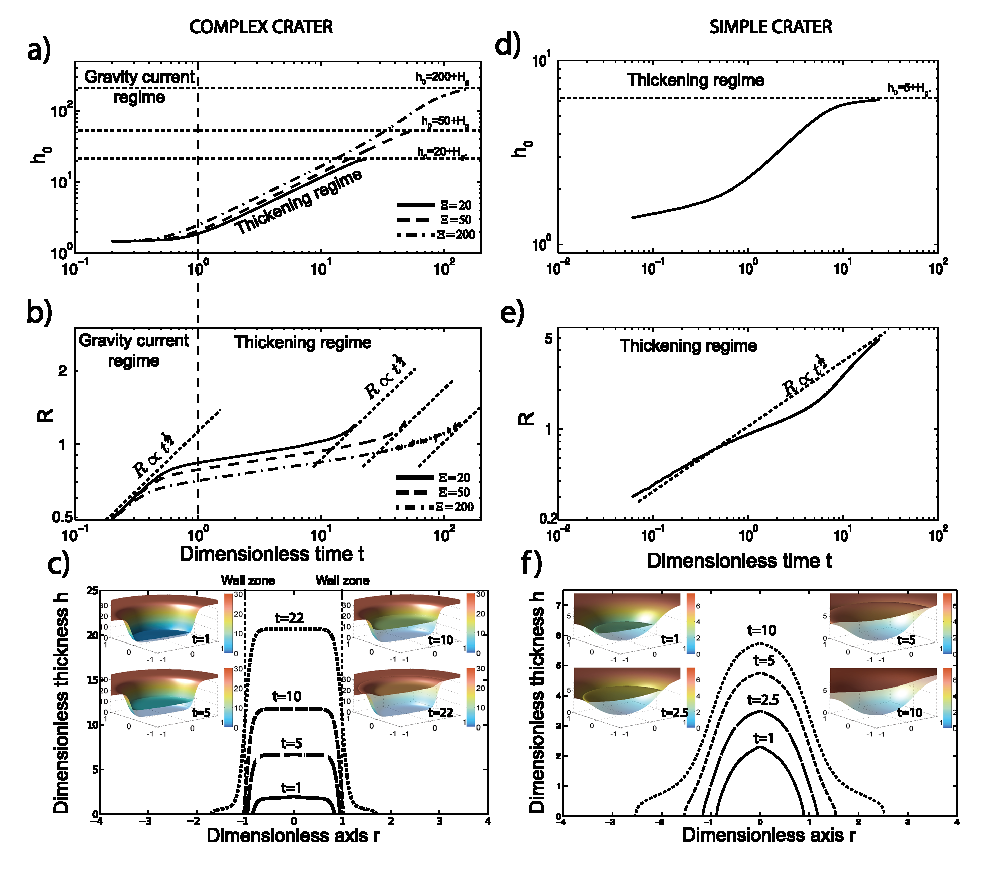
\includegraphics[scale=0.5]{fig4-2.eps}
  \caption{\textbf{a) and  b)}: Dimensionless thickness at  the center
    $h_0=h(0)$  and  edge radius  $R$  versus  dimensionless time  $t$
    \textcolor{blue}{for the case of an intrusion below a strengthless
      layer, i.e. $\Theta=0$, with a complex crater topography and for
      different values  of $\Xi$ indicated on  the graph.} Dimensional
    values are obtained by multiplying the dimensionless ones by their
    characteristic  scales  i.e.  $C$,  $H$  (\ref{eq18})  and  $\tau$
    (\ref{eq19}). The  vertical dashed line indicates  $t=1$, when the
    intrusion reaches  the wall  zone. Horizontal  dotted lines  on a)
    represent  asymptotical  behaviors  for the  different  values  of
    $\Xi$.  On b)  The dashed  lines $R\propto  t^{1/2}$ indicate  the
    scaling   law  in   the   gravity   current  regime.   \textbf{c)}
    Dimensionless intrusion profiles for  different times indicated on
    the  plot  using  $\Xi=20$.   \textcolor{blue}{For  each  time,  a
      corresponding dimensionless 3D  graph, showing the dimensionless
      floor  appearance  $T_p(r)+h(r)$,  where $T_p(r)$  is  given  by
      (\ref{TopoFinal}),  superimposed  to the  initial  dimensionless
      floor appearance  $T_p(r)$ (low opacity), is  represented to see
      the deformation induced by the intrusion on the crater floor. We
      use $\gamma=0.02$,  $\zeta=0.13$ and $\Theta=0$.  \textbf{d), e)
        and f)} Same  plots but for an intrusion  below a strengthless
      layer with a simple  crater topography, i.e. $\zeta=0.25$, using
      $\Xi=20$ only. }}
  \label{fig4-2}
\end{figure}


\begin{figure}[pb]
\graphicspath{{/Users/thorey/Documents/These/Submission/Article/FFC_JGR_2013/Paper_APRES_2nd_REVIEW/}}
  \centering
  \noindent\includegraphics[scale=0.8]{fig4-1.eps}
  \caption{\textbf{a) and  b)}: Dimensionless thickness at  the center
    $h_0=h(0)$  and  edge radius  $R$  versus  dimensionless time  $t$
    \textcolor{blue}{for  the case  of an  intrusion below  a constant
      thickness  elastic  layer.}  For  $R<4$, the  flow  dynamics  is
    controlled  by the  elastic  deformation of  the overlying  layer,
    while for a $R>4$, it is controlled  by its own weight. In a), the
    dashed   lines   correspond    to   $h_{0}\propto   t^{1/3}$   and
    $h_{0} = H_g$  which provide for scaling laws for  the elastic and
    gravity current regimes. In b) the dashed lines $R\propto t^{1/3}$
    and $R\propto t^{1/2}$ represent scaling  laws for the elastic and
    gravity current  regimes \citep{Michaut2011}. The  vertical dashed
    line indicates  the time  when the intrusion  reaches a  radius of
    $4$.  The intrusion  shape  is  shown at  different  times in  the
    elastic regime in  c) and in the gravity current  regime in d). We
    use $\gamma=0.02$, $\Xi=0$, $\Psi=0$ and $\Theta=1$. }
  \label{fig4-1}
\end{figure}

\begin{figure}[pb]
\graphicspath{{/Users/thorey/Documents/These/Submission/Article/FFC_JGR_2013/Paper_APRES_2nd_REVIEW/}}
  \centering
  \noindent\includegraphics[scale=1]{fig4-3.eps}
  \caption{Dimensionless thickness  at the center $h_0=h(0)$  and edge
    radius $R$ versus dimensionless  time $t$ \textcolor{blue}{for the
      case of an intrusion spreading  below an overlying elastic layer
      with  a   topography  characteristic   of  a   complex  crater},
    i.e. $\zeta=0.13$,  and using a constant  injection rate. Vertical
    dotted lines:  dimensionless times  when the intrusion  enters and
    leaves the thickening regime. Thick solid lines, $\Theta=10^{-2}$,
    thick dashed  lines, $\Theta=10^{-5}$.  Scaling laws are  shown in
    dash-dotted  lines for  the  elastic  regime ($R\propto  t^{1/3}$,
    $h_0\propto t ^{1/3}$) and in dotted lines for the gravity current
    regime    ($R\propto    t^{1/2}$,     $h_0    \rightarrow    H_g$,
    $h_0 \rightarrow \Xi+ H_g$).  We use, $\gamma=0.02$, $\zeta=0.13$,
    $\Xi=20$ and $\Psi=0.3$.}
  \label{fig4-3}
\end{figure}


\begin{figure}[pb]
\graphicspath{{/Users/thorey/Documents/These/Submission/Article/FFC_JGR_2013/Paper_APRES_2nd_REVIEW/}}
  \centering
  \noindent\includegraphics[scale=1]{fig4-4.eps}
  \caption{  \textbf{a) }  Profiles \textcolor{blue}{for  an intrusion
      spreading below an elastic overlying layer with a complex crater
      topography}  at  different  times  indicated  on  the  plot  for
    $\Theta=10^{-2}$, i.e.  corresponding to a small  crater and/or an
    intrusion    below   a    thick   elastic    layer.   Units    are
    dimensionless. For each time, a corresponding 3D graph showing the
    dimensionless crater floor appearance given by $T_p(r)+h(r)$ where
    $T_p(r)$ is  given by (\ref{TopoFinal}), is  represented. For each
    plot,   the   dimensionless   initial   topography   $T_p(r)$   is
    superimposed in low opacity. \textbf{b)} Same plot but for a large
    crater and/or a shallow intrusion, i.e. $\Theta=10^{-5}$. Here, we
    use $\gamma=0.02$, $\zeta=0.13$, $\Xi=20$ and $\Psi=0.3$.}
  \label{fig4-4}
\end{figure}

\begin{figure}[pb]
\graphicspath{{/Users/thorey/Documents/These/Submission/Article/FFC_JGR_2013/Paper_APRES_2nd_REVIEW/}}
  \centering
  \noindent\includegraphics[scale=0.75]{fig4-5.eps}
  \caption{   \textbf{a)}  Dimensionless   thickness  at   the  center
    $h_0=h(0)$  and edge  radius  $R$ versus  dimensionless time  $t$,
    \textcolor{blue}{for  an intrusion  spreading  below an  overlying
      layer with  a complex  crater topography},  for $\Theta=10^{-2}$
    and different values of $\Psi=0.3, 3$ and $6$. The vertical dotted
    lines indicate $t=1$, i.e. the time at which the intrusion reaches
    the wall zone. \textbf{c)}  Intrusion profiles for different times
    indicated on the plot  for $\Theta=10^{-2}$, i.e. corresponding to
    a small  crater and/or  a deep intrusion  and $\Psi=6$.  Units are
    dimensionless.  For  each  time, the  corresponding  dimensionless
    crater floor appearance given  by $T_p(r)+h(r)$, where $T_p(r)$ is
    given  by (\ref{TopoFinal}),  is represented.  For each  plot, the
    dimensionless initial  topography $T_p(r)$ is superimposed  in low
    opacity.  \textbf{e)}  Dimensionless  crater floor  appearance  at
    $t=10$ for $\Psi=6$, $\Theta=10^{-2}$. b), d) and f) Same plots as
    a),  c) and  e) but  for $\Theta=10^{-5}$.  We use  $\gamma=0.02$,
    $\zeta=0.13$ and $\Xi=20$.}
  \label{fig4-5}
\end{figure}


\begin{figure}[pb]
\graphicspath{{/Users/thorey/Documents/These/Submission/Article/FFC_JGR_2013/Paper_APRES_2nd_REVIEW/}}
  \centering
  \noindent\includegraphics[scale=0.6]{fig4-6.eps}
  \caption{  \textbf{a)}  Dimensionless   profiles,  of  an  intrusion
    spreading below  an overlying elastic  layer with a  simple crater
    topography, i.e.  $\zeta=0.25$, for different  dimensionless times
    indicated  on the  plot for  $\Theta=10^{-1}$ and  $\Psi=0.1$. For
    each  time, a  corresponding 3D  graph, showing  the dimensionless
    crater floor appearance given  by $T_p(r)+h(r)$, where $T_p(r)$ is
    given  by (\ref{TopoFinal}),  is represented.  For each  plot, the
    initial    topography   $T_p(r)$    is    superimposed   in    low
    opacity.  \textbf{b)}   Same  plot  but  for   $\Psi=4$.  We  use,
    $\gamma=0.02$ and $\Xi=20$.}
  \label{fig4-6}
\end{figure}



\begin{figure}[pb]
\graphicspath{{/Users/thorey/Documents/These/Submission/Article/FFC_JGR_2013/Paper_APRES_2nd_REVIEW/}}
  \centering
  \noindent\includegraphics[scale=0.8]{fig4-7a.eps}
  \caption{\textbf{a)}  Dimensionless   pressure  in  the   magma  $P$
    normalized by the value of  $\sigma$ versus dimensionless time $t$
    for $\Theta=10^{-2}$, for an  intrusion spreading below an elastic
    overlying layer with  a complex crater topography.  The solid line
    represents the  dimensionless pressure at  the center of  the flow
    normalized              by              $\sigma$,              i.e
    $P_{tot}/\sigma=(h_0+P_{e,r=0})/\sigma$, the dashed line indicates
    the  magma  weight  contribution $P_m/\sigma=h_0/\sigma$  and  the
    dash-dotted  line  represents  the elastic  pressure  contribution
    $P_{e,r=0}/\sigma$.  The   vertical  dotted  line   indicates  the
    dimensionless   time  when   the   intrusion   reaches  the   wall
    zone.  \textbf{b)} Initial  (dashed line)  and final,  i.e. steady
    state,    (solid   line)    dimensionless   topography    of   the
    crater. \textbf{c)} and \textbf{d)}  Same plots as \textbf{a)} and
    \textbf{b)}  but  for $\Theta=10^{-5}$.  In  c),  the dashed  line
    representing the magma weight  contribution is not distinguishable
    from the  total pressure. For  all plots, horizontal  dotted lines
    represent  asymptotic behaviors.  We use  $\gamma=0.02$, $\Xi=50$,
    $\zeta=0.13$, $\Psi=1$ and $\sigma=22$.}
  \label{fig4-7}
\end{figure}

\appendix
\numberwithin{figure}{section}
\section{Numerical scheme}
\label{AppendixA}

We use a fully implicit finite-volume method to solve (\ref{eq21}). The discretization is obtained by integrating over a finite number of non overlapping control volumes, each control volume surrounding one grid point \citep{Patankar1980}. The grid is defined by the relation $r_{i}=(i-0.5)\Delta r$ in order to avoid problems at the center. The point $b$ and $a$ define the face of the control volume surrounding $i$ such that $r_{a}=r_{i}+\Delta r/2$ and $r_{b}=r_{i}-\Delta r/2$. Because we are using an axisymmetric geometry, the control volume is an annulus of interior radius $r_b$ and exterior radius $r_a$ and its surface is $S=\pi(r_{a}^{2}-r_{b}^{2})$. Integration of (\ref{eq21}) over the control volume surrounding $i$ during a time $\Delta t$ gives:
	\begin{equation}
	\int_{t}^{t+\Delta t} \int_{r_b}^{r_a} \frac{\partial h^{*}}{\partial t} 2\pi r dr dt=\int_{t}^{t+\Delta t} \int_{b}^{a} \Phi(r,t) 2\pi r dr dt
	\label{eq27}
	 \end{equation}
 
 where $\Phi(r,t)$ stands for the right hand side of (\ref{eq21}). The classical second-order $\left (\propto \Delta r^2 \right)$ approximations is taken to derive the successive space derivatives (i.e. $\frac{\partial \Phi(r)}{\partial r}\mid_{r_a}=\frac{\Phi(i+1)-\Phi(i)}{\Delta r}$). In this way, we ensure that our final scheme is of second-order. Moreover, for more precision, the elastic pressure is calculated using a fourth-order scheme (see \ref{Fourth}.3) . In the following, we derive each term of the right hand side of (\ref{eq21}) separately, $h$ refers to the value of the thickness at  a time $t+\Delta t$ and $h^{n}$ to the value at a time $ t$.
 \subsection{Discretization}
 \label{Fourth}
 \begin{enumerate}
 \item \textbf{Time derivative}
To discretize the time derivative, we shall consider that the value of the grid point $h_{i}$ prevails throughout the control volume such that:
 \begin{equation}
 \label{num1}
 \int_{t}^{t+\Delta t} \int_{r_b}^{r_a} \frac{\partial h^{*}}{\partial t} 2\pi r dr dt=(h_{i}-h^{n}_{i})S
 \end{equation}
 \item \textbf{Gravitational term}
 \begin{eqnarray}
 \label{num2}
 \int_{t}^{t+\Delta t} \int_{r_b}^{r_a} \frac{1}{r^{*}} \frac{\partial}{\partial r^{*}}\left (r^{*} h^{3} \frac{\partial h}{\partial r^{*}} \right) 2\pi r dr dt\\
 =A^{g}_{i}h_{i+1}+B^{g}_{i}h_{i-1} -(A^{g}_{i}+B^{g}_{i})h_{i} \nonumber
 \end{eqnarray}
with $A^{g}_{i}= A=(2\pi \Delta t r_{a}h_{a}^{3})/\Delta r$ and $B^{g}_{i}=B=(2\pi \Delta t r_{b}h_{b}^{3})/\Delta r$ where the value of $h_{a}^{3}$ (resp. $h_{b}^{3}$) is approximated by $(h_{i+1}^{3}+h_{i}^{3})/2$ (resp. $(h_{i}^{3}+h_{i-1}^{3})/2$). 
 \item \textbf{Elastic term}
 	\begin{eqnarray} 
	 \label{num3}
	 \int_{t}^{t+\Delta t} \int_{r_b}^{r_a} \Theta \frac{1}{r^{*}} \frac{\partial}{\partial r^{*}}\left (r^{*} h^{3} \frac{\partial P_{e}}{\partial r^{*}} \right) 2\pi r dr dt \\
	 =A^{e}_{i}P_{e,i+1} +B^{e}_{i}P_{e,i-1 } -(A^{e}_{i}+B^{e}_{i})P_{e,i} \nonumber
	 \end{eqnarray}
	where $A^{e}_{i}= \Theta A$, $B^{e}_{i}=\Theta B$ and $P_{e}=\nabla^{2}_{r}\left( \Pi(r)\nabla^{2}_{r}h(r) \right)$, with $\Pi(r)=(1+\Psi\xi(r))^3$, is the dimensionless elastic pressure which is discretized using a fourth order finite difference scheme:}

	\begin{equation}
	 \label{num6}
	 P_{e,i}= \alpha_{i}h_{i-3} + \beta_{i}h_{i-2}+\gamma_{i} h_{i-1} +\lambda_{i}h_{i}+\kappa_{i}h_{i+1}+\delta_ih_{i+2}+\epsilon_ih_{i+3}
	\end{equation}
	with
\begin{eqnarray}
	&\alpha_{i}&=\frac{1}{24\Delta r^{4}}\left(-4p_4+3p_3\Delta_r \right)\nonumber \\
	&\beta_{i}&=\frac{1}{24\Delta r^{4}}\left(48p_4-24p_3\Delta_r-2p_2\Delta_r^2+2p_1\Delta_r^3\right) \nonumber\\
	&\gamma_{i}&=\frac{1}{24\Delta r^{4}}\left(-156p_4+39p_3\Delta_r+32p_2\Delta_r^2-16p_1\Delta_r^3\right)\nonumber\\
	&\lambda_{i}&=\frac{1}{24\Delta r^{4}}\left(224p_4-60p_2\Delta r^{2}\right) \nonumber\\
	&\kappa_{i}&=\frac{1}{24\Delta r^{4}}\left( -156p_4-39p_3\Delta_r+32p_2\Delta_r^2+16p_1\Delta_r^3\right)\nonumber\\
	&\delta_{i}&=\frac{1}{24\Delta r^{4}}\left( 48p_4+24p_3\Delta_r-2p_2\Delta_r^2-2p_1\Delta_r^3\right) \nonumber\\
	&\epsilon_{i}&=\frac{1}{24\Delta r^{4}}\left(-4p_4-3p_3\Delta_r \right)\nonumber
\end{eqnarray}
where
	\begin{eqnarray}
	p_1&=&\frac{ \Pi^{\prime\prime}_{i}}{r_i}-\frac{\Pi^{\prime}_{i}}{r_i^2} +\frac{\Pi}{r_i^3}\nonumber\\
	p_2&=&\Pi^{\prime\prime}_{i}+\frac{3\Pi^{\prime}_{i}}{r_i} +\frac{\Pi}{r_i^2}\nonumber\\
	p_3&=&2\Pi^{\prime}_{i}+\frac{2\Pi_i}{r_i}\nonumber\\
	p_4&=&\Pi_i\nonumber
	\end{eqnarray}
and where $ \Pi_{i}=(1+\Psi\xi_i)^{3}$ and $\Pi^{\prime}_{i}$ and $ \Pi^{\prime\prime}_{i}$ are its first and second derivatives with respect to the radial coordinate.
\item \textbf{Hydrostatic term}
 \begin{eqnarray}
 \label{num4}
 S^{h}_{i}= \int_{t}^{t+\Delta t} \int_{r_b}^{r_a} \Xi \frac{1}{r^{*}} \frac{\partial}{\partial r^{*}}\left (r^{*}h^{3}\frac{\partial \xi}{\partial r}\right )2\pi r dr\\
=U^{h}\left ( r_{a}h_{a}^{3} \left. \frac{\partial \xi}{\partial r}\right|_{a}-r_{b}h_{b}^{3}\left. \frac{\partial \xi}{\partial r}\right|_{b} \right )\nonumber
 \end{eqnarray}
 where $U^{h}= 2 \pi \Xi \Delta t$.
\item \textbf{Injection term}
 \begin{eqnarray}
  \label{num5}
 S^{i}_{i}&=&\int_{t}^{t+\Delta t} \int_{r_b}^{r_a} \frac{32}{\gamma^{2}} (\frac{1}{4}-\frac{r^{2}}{\gamma^{2}})  2 \pi r dr dt \\
 &=&U^{i}(\gamma^{2}-2(r_{a}^{2}+r_{b}^{2}))\nonumber
 \end{eqnarray}
 where $U^{i}=\frac{8 S \Delta t}{\gamma^{4}}$. 
 
 
 \item \textbf{Implicit scheme}
 
Substituting (\ref{num1}), (\ref{num2}), (\ref{num3}), (\ref{num4}) and (\ref{num5}) in (\ref{eq27}) and injecting (\ref{num6}), we get the final scheme given by the following equation:

\begin{equation}
a_ih_{i-4}+b_ih_{i-3}+c_ih_{i-2}+d_ih_{i-1}+e_ih_i+f_ih_{i+1}+g_ih_{i+2}+k_ih_{i+3}+l_ih_{i+4}=J_i
\label{eqd3}
\end{equation}
where the different coefficients are defined by:
\begin{eqnarray}
a_i&=&-B_i^{e}\alpha_{i-1} \\
b_i&=&(B_i^{e}+A_i^{e})\alpha_{i}-B_i^{e}\beta_{i-1} \\
c_i&=&(B_i^{e}+A_i^{e})\beta_{i}-B_i^{e}\gamma_{i-1}-A_i^{e}\alpha_{i+1} \\
d_i&=&(B_i^{e}+A_i^{e})\gamma_{i}-B_i^{e}\lambda_{i-1}-A_i^{e}\beta_{i+1} -B^{g}\\
e_i&=&S+(B_i^{e}+A_i^{e})\lambda_{i}-B_i^{e}\kappa_{i-1}-A_i^{e}\gamma_{i+1} +B^{g}+A^{g}\\
f_i&=&(B_i^{e}+A_i^{e})\kappa_{i}-B_i^{e}\delta_{i-1}-A_i^{e}\lambda_{i+1} - A^{g}\\
g_i&=&(B_i^{e}+A_i^{e})\delta_{i}-B_i^{e}\epsilon_{i-1}-A_i^{e}\kappa_{i+1} \\
k_i&=&(B_i^{e}+A_i^{e})\epsilon_{i}-A_i^{e}\delta_{i+1} \\
l_i&=&-A_i^{e}\epsilon_{i+1} \\
J_i&=&(Sh_i^n+ S^{i}_{i}+S^{h}_{i})
\end{eqnarray}	
	\subsection{Boundary conditions}
	
Since the flow is symmetric in $r=0$, we require that:
	\begin{eqnarray}
	\left.\frac{\partial h}{\partial r}\right|_{r=0}=0\\
	\left.\frac{\partial P_{e}}{\partial r}\right|_{r=0}=0
	\end{eqnarray}
 Boundary conditions at the front of the intrusion are accounted for by using a grid much larger than the intrusion where $h=0$ beyond the flow.

 \subsection{Algorithm}
The fully implicit discretization (\ref{eqd3}) can be rewritten as a linear system $\Omega(h^{3})\bar{h}=\bar{J}$ where $\bar{h}$ is a vector containing the value of $h$ a $t+\Delta t$ and $\bar{J}$ containing the right hand side of (\ref{eqd3}). The matrix $\Omega(h^{3})$ is a septadiagonal matrix and is solved by using a septadiagonal algorithm. However, due to the non-linearity of the problem (i.e. the coefficients $A_{e}, B_{e}, A_{g}$, $B_{g}$ and $S^{h}$ within the matrix $\Omega(h_{i}^{3})$ and $\bar{J}$ depend on $h_{i}^{3}$), we first have to assume values for $h_{i}$ at each grid point to inverse for the matrix and get the value of $h$ at $t+\Delta t$. We use the following iterative scheme: 
\begin{enumerate}
\item Start with a guess at all grid-point for $h_{i}=h_i^n$.
\item Calculate tentative values for the different coefficients of the system (non linear terms).
\item Apply the septadiagonal matrix algorithm to solve (\ref{eqd3}) and get a new value of $h_{i}$.
\item With this new $h_{i}$, we return to step $2$ and repeat step $2$ to $4$ until further repetitions cease to produce any significant change in $h_{i}$ (i.e. $\mid h^{new}_{i}-h_{i}\mid < \epsilon$ where $\epsilon=10^{-4}$).
\end{enumerate}
The final unchanging state is considered as the solution for the thickness of the flow at $t+\Delta t$.

\section{Elastic stresses in the upper elastic layer}
\label{AppendixB}
The stress conditions within the crater floor can be approximated using the small displacement theory. In an axisymmetric geometry, the small strain-displacement equations at the surface are:

\begin{eqnarray}
\epsilon_{rr}&=&\frac{\partial u_{r}}{\partial r}=-\frac{T_{e}(r)}{2}\frac{\partial^{2} h}{\partial r^{2}}\\
\epsilon_{\theta\theta}&=&\frac{u_{r}}{r}=-\frac{T_{e}(r)}{2r}\frac{\partial h}{\partial r} 
\end{eqnarray}

Hence, the stress conditions at the surface are given by Hooke's laws for a material under plane stress:
\begin{eqnarray}
\sigma_{rr}&=&-\frac{E T_{e}(r)}{2(1-\nu^2)}\left (\frac{\partial^{2} h}{\partial r^{2}} +\frac{\nu}{r}\frac{\partial h}{\partial r} \right)\\
\sigma_{\theta\theta}&=&-\frac{E T_{e}(r)}{2(1-\nu^2)}\left (\frac{1}{r}\frac{\partial h}{\partial r}+\nu \frac{\partial^{2}h}{\partial r^2}\right)
\end{eqnarray}

These equations are made dimensionless using the scaling of Section 3.5 where the pressure scale is $\rho_m g H$. Dimensionless radial and tangential stresses become:

\begin{eqnarray}
\sigma_{rr}&=&- \Theta \Phi \left(1+\Psi \xi(r)\right) \left ( \frac{\partial^{2} h}{\partial r^{2}} +\frac{\nu}{r}\frac{\partial h}{\partial r} \right) \\
\sigma_{\theta\theta}&=&- \Theta \Phi \left(1+\Psi \xi(r)\right) \left (\frac{1}{r}\frac{\partial h}{\partial r}+\nu \frac{\partial^{2}h}{\partial r^2}\right)
\end{eqnarray}

where $\xi(r)$ is given by (\ref{eqqqq}) and $\Phi$ is a dimensionless number given by:

\begin{equation}
\Phi= \frac{6 }{(1-\nu^2)}\left( \frac{C}{T_{e}^0} \right)^{2}
\end{equation}

The locations of the maximum stresses, where the fractures are the most likely to initiate, depend on the number $\Theta$ (Figure \ref{fig7-1} a). If the number $\Theta$ is such that $4\Lambda>>C$, i.e. $\Theta>10^{-3}$ the intrusion reaches the wall zone in an elastic regime and the maximum stresses are at the center. For $\Theta\sim10^{-3}$, $4\Lambda \sim C$ and the transition to a gravity current regime occurs at the crater wall zone. In that case, the floor is still convex but the area of maximum stress is located within a crown at a given coordinate, intermediate between the center and the wall zone, i.e. $0<r_{\sigma_{max}}<1$ (Figure \ref{fig7-1} b). Radial and tangential stresses are of the same order of magnitude. For a large crater or a shallow intrusion, i.e. a small value of the number $\Theta<10^{-3}$, the maximum stresses are concentrated within a crown adjacent to the wall zone upon the intrusion edge where the elastic deformation is important (Figure \ref{fig7-1} c ). The radial stresses that develop at the surface are generally larger than the tangential stresses favoring a circular mode of fracturing.


\begin{figure}[h!]
\begin{center} \graphicspath{{/Users/thorey/Documents/These/Submission/Article/FFC_JGR_2013/Paper_APRES_2nd_REVIEW/}}
\includegraphics[scale=0.8]{fig7-1.eps}
\caption{Solid lines: Dimensionless radial stress $\sigma_{rr}$ (top) and tangential stress $\sigma_{\theta \theta}$(bottom) at the crater floor in the case of an intrusion spreading below an overlying elastic layer with a complex crater topography for $\Theta=10^{-2}$ and $\Phi=1100$ (left), $\Theta=10^{-3}$ and $\Phi=2500$ (center) and $\Theta=10^{-5}$ and $\Phi=4500$ (right) at $t=2$. For all plots: the dotted lines represent the initial dimensionless topography $T_p(r)$ (\ref{TopoFinal}) and the dash-dotted lines represent the floor appearance $T_p(r)+h(r)$ at $t=2$. Stress is considered positive in extension. We use $\gamma=0.02$, $\Xi=20$, $\zeta=0.13$ and $\Psi=1$.}
\label{fig7-1}
\end{center}
\end{figure}

\section{Central peak}
\label{AppendixC}

Central peaks induce an increase in the lithostatic pressure as well as an increase in the overlying layer elastic thickness directly above the intrusion center. Herein, we consider an extreme case where the central peak height is one third of the crater depth and its width is one fourth of the crater size by introducing an extra gaussian function into the elastic thickness expression:

\begin{equation}
T_e(r)=T_e^0(1+\Psi(\xi(r)+C_p(r)))
\end{equation}
with
\begin{equation}
C_p(r)=50 \left(\frac{0.07}{4}\right)^2\exp\left(-\frac{r^2}{2(\frac{0.07}{4})^2}\right)
\end{equation}

For a strengthless overlying layer and $\Theta=0$ (Section  \ref{Strengthless_Layer1} equation (\ref{eq22})), the central peak only adds an excess in lithostatic pressure at the center of the crater floor. In response, the intrusion preferentially develops around the central peak and then spreads until it reaches the crater wall (Figure \ref{fig7-2} a). At the crater wall, the lithostatic pressure increase induces the thickening of the intrusion. However, due to the excess of lithostatic pressure at the center, the center of the intrusion below the central peak does not thickens and the thickening only concerns an annulus located in between the central peak and the crater wall (Figure \ref{fig7-2} a). At the surface, the central peak height decreases until the thickening is important enough to compensate for the initial excess in lithostatic pressure. A balance between the two pressures gives the final height of the central peak, equal to the initial height times $(\rho_m-\rho_c)/\rho_m$ (Figure \ref{fig7-2} a). Next, the resulting central peak is just leveled up with the whole crater floor. 

For an elastic overlying layer such that $\Theta=10^{-5}$, the inner part of the intrusion adjacent to the central peak is bent by the weight of the central peak. As a consequence, during the thickening stage, a second circular moat, whose size is $4\Lambda$, arises and borders the central peak. As previously, the central peak height decreases until the sum of the elastic and hydrostatic pressure compensate for the initial excess of lithostatic pressure due to the central peak and is then leveled up during floor uplift.

Finally, in the case of a thick elastic overlying layer, i.e. a large value of $\Theta$, the flexural wavelength is almost not affected by the presence of the central peak and the central peak is leveled up with the convex floor during crater floor uplift (Figure \ref{fig7-2} c).


\begin{figure}[h!]
\begin{center}
\graphicspath{{/Users/thorey/Documents/These/Submission/Article/FFC_JGR_2013/Paper_APRES_2nd_REVIEW/ }}
 \includegraphics[scale=0.55]{fig7-2.eps}
 \caption{ \textbf{a)} Dimensionless intrusion profiles for different dimensionless times indicated on the plot for $\Psi=4$ and for an intrusion spreading below a strengthless overlying layer with a complex crater topography and a central peak i.e. $\Theta=0$ and  $\zeta=0.13$. For each time, a corresponding 3D graph, showing the dimensionless crater floor appearance given by $T_p(r)+h(r)$ where, here, $T_p(r)=\Xi \Omega(\xi(r)+C_p(r))$, is represented. For each plot, the initial topography given by $T_p(r)=\Xi \Omega(\xi(r)+C_p(r))$ is superimposed in low opacity. \textbf{b)} Same plot but for an overlying elastic layer such that $\Theta=10^{-5}$. \textbf{c)} Same plot but for an elastic overlying layer such that $\Theta=10^{-2}$. Here we use, $\gamma=0.02$, $\Xi=20$ and $\Psi=4$.}
\label{fig7-2}
\end{center}
\end{figure}

\newpage

%
% ACKNOWLEDGMENTS

\begin{acknowledgments}
	The authors are grateful to R. W. Wichman and P. H. Schultz for their thoughtful comments and careful reviews. This work was supported by PNP/INSU and by Labex UNIVEARTH, Universit\'e Paris Diderot.
\end{acknowledgments}

\bibliographystyle{agufull08.bst}
\begin{thebibliography}{39}
\providecommand{\natexlab}[1]{#1}
\expandafter\ifx\csname urlstyle\endcsname\relax
  \providecommand{\doi}[1]{doi:\discretionary{}{}{}#1}\else
  \providecommand{\doi}{doi:\discretionary{}{}{}\begingroup
  \urlstyle{rm}\Url}\fi

\bibitem[{\textit{Baker et~al.}(2012)\textit{Baker, Head, Neumann, Smith, and
  Zuber}}]{Baker2012}
Baker, D. M.~H., J.~W. Head, G.~A. Neumann, D.~E. Smith, and M.~T. Zuber
  (2012), {The transition from complex craters to multi-ring basins on the
  Moon: Quantitative geometric properties from Lunar Reconnaissance Orbiter
  Lunar Orbiter Laser Altimeter (LOLA) data}, \textit{Journal of Geophysical
  Research: Planets}, \textit{117}(E3), \doi{10.1029/2011JE004021}.

\bibitem[{\textit{Bray et~al.}(2008)\textit{Bray, Collins, Morgan, and
  Sschenk}}]{BRAY2008a}
Bray, V.~J., G.~S. Collins, J.~V. Morgan, and P.~M. Sschenk (2008), {The effect
  of target properties on crater morphology: Comparison of central peak craters
  on the Moon and Ganymede}, \textit{Meteoritics \& Planetary Science},
  \textit{43}(12), 1979--1992, \doi{10.1111/j.1945-5100.2008.tb00656.x}.

\bibitem[{\textit{Bunger and Cruden}(2011)}]{Bunger2011}
Bunger, A.~P., and A.~R. Cruden (2011), {Modeling the growth of laccoliths and
  large mafic sills: Role of magma body forces}, \textit{Journal of Geophysical
  Research: Solid Earth}, \textit{116}(B2), \doi{10.1029/2010JB007648}.

\bibitem[{\textit{Crisp}(1984)}]{Crisp1984}
Crisp, J.~A. (1984), {Rates of magma emplacement and volcanic output},
  \textit{Journal of Volcanology and Geothermal Research}, \textit{20}(3),
  177--211, \doi{10.1016/0377-0273(84)90039-8}.

\bibitem[{\textit{Dombard and Gillis}(2001)}]{Dombard2001}
Dombard, A.~J., and J.~J. Gillis (2001), {Testing the viability of topographic
  relaxation as a mechanism for the formation of lunar floor-fractured
  craters}, \textit{Journal of Geophysical Research: Planets},
  \textit{106}(E11), 27,901--27,909, \doi{10.1029/2000JE001388}.

\bibitem[{\textit{El-Baz}(1970)}]{El-Baz1970}
El-Baz, F. (1970), {Lunar igneous intrusions.}, \textit{Science},
  \textit{167}(3914), 49--50.

\bibitem[{\textit{Glotch et~al.}(2010)\textit{Glotch, Lucey, Bandfield,
  Greenhagen, Thomas, Elphic, Bowles, Wyatt, Allen, {Donaldson Hanna}, and
  Paige}}]{Glotch2010}
Glotch, T.~D., P.~G. Lucey, J.~L. Bandfield, B.~T. Greenhagen, I.~R. Thomas,
  R.~C. Elphic, N.~Bowles, M.~B. Wyatt, C.~C. Allen, K.~{Donaldson Hanna}, and
  D.~A. Paige (2010), {Highly silicic compositions on the Moon.},
  \textit{Science}, \textit{329}(5998), 1510--3, \doi{10.1126/science.1192148}.

\bibitem[{\textit{Hall et~al.}(1981)\textit{Hall, Solomon, and
  Head}}]{Hall1981a}
Hall, J.~L., S.~C. Solomon, and J.~W. Head (1981), {Lunar floor-fractured
  craters: Evidence for viscous relaxation of crater topography},
  \textit{Journal of Geophysical Research: Solid Earth}, \textit{86}(B10),
  9537--9552, \doi{10.1029/JB086iB10p09537}.

\bibitem[{\textit{Head and Wilson}(1992)}]{Head1992a}
Head, J.~W., and L.~Wilson (1992), {Lunar mare volcanism: Stratigraphy,
  eruption conditions, and the evolution of secondary crusts},
  \textit{Geochimica et Cosmochimica Acta}, \textit{56}(6), 2155--2175,
  \doi{10.1016/0016-7037(92)90183-J}.

\bibitem[{\textit{Head et~al.}(2009)\textit{Head, Murchie, Prockter, Solomon,
  Chapman, Strom, Watters, Blewett, Gillis-Davis, Fassett, Dickson, Morgan, and
  Kerber}}]{Head2009a}
Head, J.~W., S.~L. Murchie, L.~M. Prockter, S.~C. Solomon, C.~R. Chapman, R.~G.
  Strom, T.~R. Watters, D.~T. Blewett, J.~J. Gillis-Davis, C.~I. Fassett, J.~L.
  Dickson, G.~a. Morgan, and L.~Kerber (2009), {Volcanism on Mercury: Evidence
  from the first MESSENGER flyby for extrusive and explosive activity and the
  volcanic origin of plains}, \textit{Earth and Planetary Science Letters},
  \textit{285}(3), 227--242, \doi{10.1016/j.epsl.2009.03.007}.

\bibitem[{\textit{Hiesinger and Head}(2006)}]{Hiesinger2006}
Hiesinger, H., and J.~W. Head (2006), {New Views of Lunar Geoscience: An
  Introduction and Overview}, \textit{Reviews in Mineralogy and Geochemistry},
  \textit{60}(1), 1--81, \doi{10.2138/窶脚mg.2006.60.1}.

\bibitem[{\textit{Huppert}(1982)}]{Huppert1982}
Huppert, H.~E. (1982), {The propagation of two-dimensional and axisymmetric
  viscous gravity currents over a rigid horizontal surface}, \textit{Journal of
  Fluid Mechanics}, \textit{121}(1), 43--58, \doi{10.1017/S0022112082001797}.

\bibitem[{\textit{Johnson and Pollard}(1973)}]{Johnson1973}
Johnson, A.~M., and D.~D. Pollard (1973), {Mechanics of growth of some
  laccolithic intrusions in the Henry mountains, Utah, I},
  \textit{Tectonophysics}, \textit{18}(3), 261--309,
  \doi{10.1016/0040-1951(73)90050-4}.

\bibitem[{\textit{Jolliff et~al.}(2000)\textit{Jolliff, Gaddis, Ryder, Neal,
  Shearer, Elphic, Johnson, Keller, Kerotev, and Lawrence}}]{Jolliff2000}
Jolliff, B.~L., L.~R. Gaddis, G.~Ryder, C.~R. Neal, C.~K. Shearer, R.~C.
  Elphic, J.~R. Johnson, L.~P. Keller, R.~L. Kerotev, and D.~J. Lawrence
  (2000), {New views of the Moon: Improved understanding through data
  integration}, \textit{Eos, Transactions American Geophysical Union},
  \textit{81}(31), 349--355.

\bibitem[{\textit{Jozwiak et~al.}(2012)\textit{Jozwiak, Head, Zuber, Smith, and
  Neumann}}]{Jozwiak2012}
Jozwiak, L.~M., J.~W. Head, M.~T. Zuber, D.~E. Smith, and G.~A. Neumann (2012),
  {Lunar floor-fractured craters: Classification, distribution, origin and
  implications for magmatism and shallow crustal structure}, \textit{Journal of
  Geophysical Research: Planets}, \textit{117}(E11),
  \doi{10.1029/2012JE004134}.

\bibitem[{\textit{Kalynn et~al.}(2013)\textit{Kalynn, Johnson, Osinski, and
  Barnouin}}]{Kalynn2013a}
Kalynn, J., C.~L. Johnson, G.~R. Osinski, and O.~Barnouin (2013), {Topographic
  characterization of lunar complex craters}, \textit{Geophysical Research
  Letters}, \textit{40}(1), 38--42, \doi{10.1029/2012GL053608}.

\bibitem[{\textit{Laneuville et~al.}(2013)\textit{Laneuville, Wieczorek,
  Breuer, and Tosi}}]{Laneuville2013}
Laneuville, M., M.~A. Wieczorek, D.~Breuer, and N.~Tosi (2013), {Asymmetric
  thermal evolution of the Moon}, \textit{Journal of Geophysical Research:
  Planets}, \textit{118}(7), 1435--1452, \doi{10.1002/jgre.20103}.

\bibitem[{\textit{Melosh}(1989)}]{Melosh1989}
Melosh, H.~J. (1989), {Impact cratering: A geologic process}, \textit{Research
  supported by NASA. New York, Oxford University Press (Oxford Monographs on
  Geology and Geophysics, No. 11), 1989, 253 p.}, \textit{1}.

\bibitem[{\textit{Michaut}(2011)}]{Michaut2011}
Michaut, C. (2011), {Dynamics of magmatic intrusions in the upper crust: Theory
  and applications to laccoliths on Earth and the Moon}, \textit{Journal of
  Geophysical Research: Solid Earth}, \textit{116}(B5),
  \doi{10.1029/2010JB008108}.

\bibitem[{\textit{Michaut and Bercovici}(2009)}]{Michaut2009}
Michaut, C., and D.~Bercovici (2009), {A model for the spreading and compaction
  of two-phase viscous gravity currents}, \textit{Journal of Fluid Mechanics},
  \textit{630}, 299, \doi{10.1017/S0022112009006612}.

\bibitem[{\textit{Michaut et~al.}(2013)\textit{Michaut, Baratoux, and
  Thorey}}]{Michaut2013}
Michaut, C., D.~Baratoux, and C.~Thorey (2013), {Magmatic intrusions and
  deglaciation at mid-latitude in the northern plains of Mars},
  \textit{Icarus}, \textit{225}(1), 602--613,
  \doi{10.1016/j.icarus.2013.04.015}.

\bibitem[{\textit{O'Keefe and Ahrens}(1999)}]{O'Keefe1999}
O'Keefe, J.~D., and T.~J. Ahrens (1999), {Complex craters: Relationship of
  stratigraphy and rings to impact conditions}, \textit{Journal of Geophysical
  Research: Planets}, \textit{104}(E11), 27,091--27,104,
  \doi{10.1029/1998JE000596}.

\bibitem[{\textit{Patankar}(1980)}]{Patankar1980}
Patankar, S.~V. (1980), \textit{{Numerical heat transfer and fluid flow}},
  Series in computational and physical processes in mechanics and thermal
  sciences, Hemisphere Publishing Company.

\bibitem[{\textit{Pike}(1974)}]{Pike1974}
Pike, R.~J. (1974), {Depth/diameter relations of fresh lunar craters: Revision
  from spacecraft data}, \textit{Geophysical Research Letters}, \textit{1}(7),
  291--294, \doi{10.1029/GL001i007p00291}.
  
  \bibitem[{\textit{Pike}(1976)}]{Pike1976}
Pike, R. (1976), {Crater dimensions from Apollo data and supplemental sources},
  \textit{The Moon}, \textit{15}(3-4), 463--477.

\bibitem[{\textit{Pike}(1980)}]{Pike1980}
Pike, R.~J. (1980), {Formation of complex impact craters:
  Evidence from Mars and other planets}, \textit{Icarus}, \textit{43}(1),
  1--19, \doi{10.1016/0019-1035(80)90083-4}.

\bibitem[{\textit{Pollard and Johnson}(1973)}]{Pollard1973a}
Pollard, D.~D., and A.~M. Johnson (1973), {Mechanics of growth of some
  laccolithic intrusions in the Henry mountains, Utah, II: Bending and failure
  of overburden layers and sill formation}, \textit{Tectonophysics},
  \textit{18}(3), 311--354, \doi{0040-1951(73)90051-6}.

\bibitem[{\textit{Rivalta et~al.}(2005)\textit{Rivalta, B\"{o}ttinger, and
  Dahm}}]{Rivalta2005}
Rivalta, E., M.~B\"{o}ttinger, and T.~Dahm (2005), {Buoyancy-driven fracture
  ascent: Experiments in layered gelatine}, \textit{Journal of Volcanology and
  Geothermal Research}, \textit{144}(1-4), 273--285,
  \doi{10.1016/j.jvolgeores.2004.11.030}.

\bibitem[{\textit{Sato et~al.}(2010)\textit{Sato, Kurita, and
  Baratoux}}]{Sato2010}
Sato, H., K.~Kurita, and D.~Baratoux (2010), {The formation of floor-fractured
  craters in Xanthe Terra}, \textit{Icarus}, \textit{207}(1), 248--264,
  \doi{10.1016/j.icarus.2009.10.023}.

\bibitem[{\textit{Schultz}(1976{\natexlab{a}})}]{Schultz1976}
Schultz, P.~H. (1976{\natexlab{a}}), {Floor-fractured lunar craters},
  \textit{The Moon}, \textit{15}(3-4), 241--273, \doi{10.1007/BF00562240}.

\bibitem[{\textit{Schultz}(1976{\natexlab{b}})}]{Schultz1976a}
Schultz, P.~H. (1976{\natexlab{b}}), {Moon morphology: Interpretations based on
  Lunar Orbiter photography}, \textit{University of Texas Press}, \textit{1}.

\bibitem[{\textit{Schultz}(1978)}]{Schultz1978}
Schultz, P.~H. (1978), {Martian intrusions: Possible sites and implications},
  \textit{Geophysical Research Letters}, \textit{5}(6), 457--460,
  \doi{10.1029/GL005i006p00457}.

\bibitem[{\textit{Schultz}(1988)}]{Schultz1988}
Schultz, P.~H. (1988), {Cratering on Mercury: A relook}, \textit{Mercury}, pp.
  274--335.

\bibitem[{\textit{Schultz and Glicken}(1979)}]{Schultz1979}
Schultz, P.~H., and H.~Glicken (1979), {Impact crater and basin control of
  igneous processes on Mars}, \textit{Journal of Geophysical Research},
  \textit{84}(B14), 8033, \doi{10.1029/JB084iB14p08033}.

\bibitem[{\textit{Schultz et~al.}(1994)\textit{Schultz, Koeberl, Bunch, Grant,
  and Collins}}]{Schultz1994}
Schultz, P.~H., C.~Koeberl, T.~Bunch, J.~Grant, and W.~Collins (1994), {Ground
  truth for oblique impact processes: New insight from the Rio Cuarto,
  Argentina, crater field}, \textit{Geology}, \textit{22}(10), 889--892.

\bibitem[{\textit{Taisne and Tait}(2009)}]{Taisne2009a}
Taisne, B., and S.~Tait (2009), {Eruption versus intrusion? Arrest of
  propagation of constant volume, buoyant, liquid-filled cracks in an elastic,
  brittle host}, \textit{Journal of Geophysical Research}, \textit{114}(B6),
  \doi{10.1029/2009JB006297}.

\bibitem[{\textit{Turcotte et~al.}(1981)\textit{Turcotte, Willemann, Haxby, and
  Norberry}}]{Turcotte1981}
Turcotte, D.~L., R.~J. Willemann, W.~F. Haxby, and J.~Norberry (1981), {Role of
  membrane stresses in the support of planetary topography}, \textit{Journal of
  Geophysical Research}, \textit{86}(B5), 3951--3959,
  \doi{10.1029/JB086iB05p03951}.
 
\bibitem[{\textit{Walker}(1989)}]{Walker1989}
Walker, G. (1989), {Gravitational (density) controls on volcanism, magma chambers and intrusions}, \textit{Australian Journal of Earth Sciences},
  \textit{36}(2), 149-165, \doi{10.1080/08120098908729479}.

\bibitem[{\textit{Wichman and Schultz}(1993)}]{Wichman1993}
Wichman, R.~W., and P.~H. Schultz (1993), {Floor-fractured crater models of the
  Sudbury Structure, Canada: Implications for initial crater size and crater
  modification}, \textit{Meteoritics}, \textit{28}(2), 222--231,
  \doi{10.1111/j.1945-5100.1993.tb00760.x}.

\bibitem[{\textit{Wichman and Schultz}(1995{\natexlab{a}})}]{Wichman1995a}
Wichman, R.~W., and P.~H. Schultz (1995{\natexlab{a}}), {Floor-fractured impact
  craters on Venus: Implications for igneous crater modification and local
  magmatism}, \textit{Journal of Geophysical Research},
  \textit{100}(E2), 3233--3244, \doi{10.1029/94JE03206}.

\bibitem[{\textit{Wichman and Schultz}(1995{\natexlab{b}})}]{Wichman1995b}
Wichman, R.~W., and P.~H. Schultz (1995{\natexlab{b}}), {Floor-fractured
  craters in Mare Smythii and west of Oceanus Procellarum: Implications of
  crater modification by viscous relaxation and igneous intrusion models},
  \textit{Journal of Geophysical Research}, \textit{100}(E10), 21,201-- 21,218,
  \doi{10.1029/95JE02297}.

\bibitem[{\textit{Wichman and Schultz}(1996)}]{Wichman1996}
Wichman, R.~W., and P.~H. Schultz (1996), {Crater-Centered Laccoliths on the
  Moon: Modeling Intrusion Depth and Magmatic Pressure at the Crater
  Taruntius}, \textit{Icarus}, \textit{122}(1), 193--199,
  \doi{10.1006/icar.1996.0118}.

\bibitem[{\textit{Wieczorek et~al.}(2001)\textit{Wieczorek, Zuber, and
  Phillips}}]{Wieczorek2001}
Wieczorek, M.~A., M.~T. Zuber, and R.~J. Phillips (2001), {The role of magma
  buoyancy on the eruption of lunar basalts}, \textit{Earth and Planetary
  Science Letters}, \textit{185}(1), 71--83,
  \doi{10.1016/S0012-821X(00)00355-1}.

\bibitem[{\textit{Wieczorek et~al.}(2013)\textit{Wieczorek, Neumann, Nimmo,
  Kiefer, Taylor, Melosh, Phillips, Solomon, Andrews-Hanna, Asmar, Konopliv,
  Lemoine, Smith, Watkins, Williams, and Zuber}}]{Wieczorek2012}
Wieczorek, M.~a., G.~a. Neumann, F.~Nimmo, W.~S. Kiefer, G.~J. Taylor, H.~J.
  Melosh, R.~J. Phillips, S.~C. Solomon, J.~C. Andrews-Hanna, S.~W. Asmar,
  A.~S. Konopliv, F.~G. Lemoine, D.~E. Smith, M.~M. Watkins, J.~G. Williams,
  and M.~T. Zuber (2013), {The Crust of the Moon as Seen by GRAIL.},
  \textit{Science}, \textit{339}(6120), 671--675,
  \doi{10.1126/science.1231530}.

\bibitem[{\textit{Wilhelms et~al.}(1987)\textit{Wilhelms, McCauley, and
  Trask}}]{Wilhelms1987a}
Wilhelms, D.~E., J.~F. McCauley, and N.~J. Trask (1987), {The geologic history
  of the Moon}.

\bibitem[{\textit{Wilson and Head}(1981)}]{Wilson1981}
Wilson, L., and J.~W. Head (1981), {Ascent and eruption of basaltic magma on
  the Earth and Moon}, \textit{Journal of Geophysical Research},
  \textit{86}(B4), 2971--3001, \doi{10.1029/JB086iB04p02971}.

\end{thebibliography}

\newpage 

\begin{table}
	\caption{A summary of Floor-Fractured Craters classification as proposed by \citet{Jozwiak2012} following \citet{Schultz1976}}
	\centering
	 \begin{tabular}{c|c}
	 \hline
	 Class & Description \\
	 \hline

	 1 & Large craters: $50-300$ km (average $140$ km)\\
	    & Deep floor \\
	    & Absence of moats\\
	    & Radial or concentric fractures\\
	  \hline
	 2 & Mid-size craters: $13-75$ km (mean $30$ km)\\
	  		 & Shallow convex floor \\
			 & Absence of moats\\
			 & Strong concentric fractures\\
			 \hline
	 3 & $12-170$ km (mean $50$ km)\\
	  		& Shallow central flat floor\\
			& Wide U-Shaped moat\\
			& Radial or polygonal fractures\\
	 \hline
	4a & Small craters: $4-38$ km (mean $15$km)\\
	 	   & Shallow convex floor \\
		   & Weak V-shaped moat\\
		   & Strong radial and concentric fractures \\
		    \hline
	 4b & Small craters: $7-45$ km (average:$25$km)\\
	  	     & Shallow convex floor \\
		     & Pronounced V-shaped moat + inner ridges\\
		     & Subtle radial fractures\\
		     \hline
     4c & Small craters: average $15$ km \\
      		& Flat or concave up floor \\
			& V-shaped moats \\
			& Hummocky, lack of fracture \\
			\hline
	5 & Large craters: $12-177$ km (average $70$km)\\
	 	    & Shallow old and degraded central flat floor\\
		    & Absence of moats \\
		    & Strong radial, concentric and/or polygonal fractures\\
		    \hline
	6 & Large craters: $50-200$km \\
	 	    & Completely flooded by basalt\\
		    & Absence of moats\\
		    & Concentric fractures
		        \label{tab1}
	\end{tabular} 
	 %\tablenotetext{a}{Footnote text here.}
	 \end{table}
	

	\begin{table}
	\caption{Range of values for the model parameters}
	\centering
	 \begin{tabular}{c|c|c}
	 \hline
	 Parameters& Symbol & Range of values \\
	 \hline
	 &&\\
	 Depth of intrusion & $T_{e}^0$ & $0.5-5$ km \\
	 Young's Modulus & $E$ & $1-10$ GPa \\
	 Poisson's ratio & $\nu$ & $0.25$ \\
	 Gravity & $g$ & $1.62$ m.s$^{-2}$ \\
	 Magma density & $\rho_{m}$ & $2800-3200$ kg.m$^{-3}$ \\
	 Magma viscosity & $\mu $ & $1-10^{4}$ Pa.s -\\
	 Feeder dyke width & $ a$ & $10-100$ m \\
	Depth of the melt source & $Z_{c}$ & $ 200-500$ km \\ 
	Initial overpressure & $\Delta P$ & $1-20$ MPa \\
	Injection rate & $Q_{0}$ &$0.1-2.10^8$ m$^{3}$.s$^{-1}$ \\
	Crust density & $\rho_{c}$ & $2500$ kg.m$^{-3}$ \\
	Crater depth & $D_{c}$ & $500-4000$ m \\
	&&\\
	\hline
	 Characteristic scales & Symbol & Range of values \\
	 \hline
	 &&\\
	Height scale & $H$& $1-35$ m \\
	Length scale & $C$    & $1-50$ km \\
	Time scale & $\tau$ & $10^{-3}-1$ years \\
	Flexural wavelength & $\Lambda$ & $1-12$ km 
	 \label{tab2}
	\end{tabular} 
	 \end{table}
	 
	 
	\begin{table}
	\caption{Dimensionless numbers}
	\centering
	 \begin{tabular}{c|c|c|c}
	 &&Complex craters&Simple craters \\
	 \hline
      Symbol& Description & Range of values & Range of values \\
	\hline
	&&\\
	$\gamma$&Normalized source width& $10^{-4}-10^{-2}$ &$10^{-4}-10^{-2}$ \\
	$\zeta$& Normalized wall zone width  & $0.05-0.13$&$0.25$\\
	 $\Psi$&Thickening term & $0.3-8$&$0.2-4$\\
	 $\Xi$& Hydrostatic term & $20-400$&$20-200$\\
	$\Theta$ &Elastic term & $10^{-7}-0.1$&$10^{-3}-10$\\
	$\Omega$ & Density ratio & $1.2$ &$1.2$\\
	$\Phi$ & Upper layer aspect ratio & $4500$ &$1200 $\\
	$\sigma$&Normalized pressure head& $0.6-100$ & $0.6-100$ 
     \label{tab3}
	\end{tabular} 
	 %\tablenotetext{a}{Footnote text here.}
	 \end{table}
	 


%%% Local Variables:
%%% mode: latex
%%% TeX-master: "../main"
%%% End:
